\documentclass[twoside]{book}

% Packages required by doxygen
\usepackage{fixltx2e}
\usepackage{calc}
\usepackage{doxygen}
\usepackage[export]{adjustbox} % also loads graphicx
\usepackage{graphicx}
\usepackage[utf8]{inputenc}
\usepackage{makeidx}
\usepackage{multicol}
\usepackage{multirow}
\PassOptionsToPackage{warn}{textcomp}
\usepackage{textcomp}
\usepackage[nointegrals]{wasysym}
\usepackage[table]{xcolor}

% NLS support packages
Portuguese
% Font selection
\usepackage[T1]{fontenc}
\usepackage[scaled=.90]{helvet}
\usepackage{courier}
\usepackage{amssymb}
\usepackage{sectsty}
\renewcommand{\familydefault}{\sfdefault}
\allsectionsfont{%
  \fontseries{bc}\selectfont%
  \color{darkgray}%
}
\renewcommand{\DoxyLabelFont}{%
  \fontseries{bc}\selectfont%
  \color{darkgray}%
}
\newcommand{\+}{\discretionary{\mbox{\scriptsize$\hookleftarrow$}}{}{}}

% Page & text layout
\usepackage{geometry}
\geometry{%
  a4paper,%
  top=2.5cm,%
  bottom=2.5cm,%
  left=2.5cm,%
  right=2.5cm%
}
\tolerance=750
\hfuzz=15pt
\hbadness=750
\setlength{\emergencystretch}{15pt}
\setlength{\parindent}{0cm}
\setlength{\parskip}{3ex plus 2ex minus 2ex}
\makeatletter
\renewcommand{\paragraph}{%
  \@startsection{paragraph}{4}{0ex}{-1.0ex}{1.0ex}{%
    \normalfont\normalsize\bfseries\SS@parafont%
  }%
}
\renewcommand{\subparagraph}{%
  \@startsection{subparagraph}{5}{0ex}{-1.0ex}{1.0ex}{%
    \normalfont\normalsize\bfseries\SS@subparafont%
  }%
}
\makeatother

% Headers & footers
\usepackage{fancyhdr}
\pagestyle{fancyplain}
\fancyhead[LE]{\fancyplain{}{\bfseries\thepage}}
\fancyhead[CE]{\fancyplain{}{}}
\fancyhead[RE]{\fancyplain{}{\bfseries\leftmark}}
\fancyhead[LO]{\fancyplain{}{\bfseries\rightmark}}
\fancyhead[CO]{\fancyplain{}{}}
\fancyhead[RO]{\fancyplain{}{\bfseries\thepage}}
\fancyfoot[LE]{\fancyplain{}{}}
\fancyfoot[CE]{\fancyplain{}{}}
\fancyfoot[RE]{\fancyplain{}{\bfseries\scriptsize Gerado por Doxygen }}
\fancyfoot[LO]{\fancyplain{}{\bfseries\scriptsize Gerado por Doxygen }}
\fancyfoot[CO]{\fancyplain{}{}}
\fancyfoot[RO]{\fancyplain{}{}}
\renewcommand{\footrulewidth}{0.4pt}
\renewcommand{\chaptermark}[1]{%
  \markboth{#1}{}%
}
\renewcommand{\sectionmark}[1]{%
  \markright{\thesection\ #1}%
}

% Indices & bibliography
\usepackage{natbib}
\usepackage[titles]{tocloft}
\setcounter{tocdepth}{3}
\setcounter{secnumdepth}{5}
\makeindex

% Hyperlinks (required, but should be loaded last)
\usepackage{ifpdf}
\ifpdf
  \usepackage[pdftex,pagebackref=true]{hyperref}
\else
  \usepackage[ps2pdf,pagebackref=true]{hyperref}
\fi
\hypersetup{%
  colorlinks=true,%
  linkcolor=blue,%
  citecolor=blue,%
  unicode%
}

% Custom commands
\newcommand{\clearemptydoublepage}{%
  \newpage{\pagestyle{empty}\cleardoublepage}%
}

\usepackage{caption}
\captionsetup{labelsep=space,justification=centering,font={bf},singlelinecheck=off,skip=4pt,position=top}

%===== C O N T E N T S =====

\begin{document}

% Titlepage & ToC
\hypersetup{pageanchor=false,
             bookmarksnumbered=true,
             pdfencoding=unicode
            }
\pagenumbering{alph}
\begin{titlepage}
\vspace*{7cm}
\begin{center}%
{\Large Sistema de Alocação de Demanda de Transporte }\\
\vspace*{1cm}
{\large Gerado por Doxygen 1.8.13}\\
\end{center}
\end{titlepage}
\clearemptydoublepage
\pagenumbering{roman}
\tableofcontents
\clearemptydoublepage
\pagenumbering{arabic}
\hypersetup{pageanchor=true}

%--- Begin generated contents ---
\chapter{Trabalho Prático P\+DS II}
\label{md_README}
\Hypertarget{md_README}
Trabalho prático (TP) de {\bfseries Programação e Desenvolvimento de Software II (D\+C\+C204)} da {\bfseries U\+F\+MG} em 2019/2.

Professor\+: Júlio César()

\subsection*{Sistema de Alocação de Demanda de Transporte}

$\vert$ \href{#introdução}{\tt Introdução} $\vert$ \href{#integrantes}{\tt Integrantes} $\vert$ \href{#documentação}{\tt Documentação} $\vert$\href{#slides}{\tt Slides} $\vert$ \href{#user-stories}{\tt User Stories} $\vert$ \href{#como-usar}{\tt Como usar} $\vert$ $\vert$ -\/-\/-\/-\/-\/-\/-\/-\/--- $\vert$ -\/-\/-\/-\/-\/-\/-\/-\/-\/-\/-\/--- $\vert$ -\/-\/-\/-\/-\/-\/-\/-\/-\/-\/-\/--- $\vert$ -\/-\/-\/-\/-\/-\/-\/-\/--- $\vert$ -\/-\/-\/-\/-\/-\/-\/-\/--- $\vert$ -\/-\/-\/-\/-\/-\/-\/-\/--- $\vert$ 



\subsubsection*{Introdução}

Este Trabalho Prático consiste no desenvolvimento de um sistema em linguagem C++ baseado no paradigma de Orientação à Objetos. Para modelar um sistema de alocação de demanda de transporte utilizamos de classes abstratas e conceitos de OO como modularização, polimorfismo, testes de unidade e boas práticas de programação em geral como refatoração, código comentado e versionamento de código.

Desenvolvemos, portanto, um sistema que, dada uma demanda de transporte de uma certa quantidade de determinado produto, para alguma localidade do Brasil ou Exterior, encontra o caminho de menor custo. O custo a ser considerado pode ser monetário ou menor distância ou tempo de percurso, considerando os preços dos serviços, tempo de transporte e capacidade dos diversos modais disponíveis (rodoviário, ferroviário, aéreo e aquaviário).

\subsubsection*{Integrantes}


\begin{DoxyItemize}
\item Estevão de Almeida Vilela ()
\item Wagner Abreu ()
\end{DoxyItemize}

\subsubsection*{Documentação}

Disponível \mbox{[}aqui\mbox{]}() em P\+DF

\subsubsection*{Slides}

Disponível \mbox{[}aqui\mbox{]}() em P\+PT

\subsubsection*{User Stories}

Disponível \mbox{[}aqui\mbox{]}()

\subsubsection*{Como usar}

O usuário do sistema deve inserir a quantidade de carga que deseja transportar entre duas localidades disponíveis. As localidades que estão disponíveis são as capitais do Brasil e algumas capitais de países estrangeiros. 
\chapter{Índice da hierarquia}
\section{Hierarquia de classes}
Esta lista de heranças está organizada, dentro do possível, por ordem alfabética\+:\begin{DoxyCompactList}
\item \contentsline{section}{Localidade}{\pageref{classLocalidade}}{}
\item \contentsline{section}{Modal}{\pageref{classModal}}{}
\begin{DoxyCompactList}
\item \contentsline{section}{Aereo}{\pageref{classAereo}}{}
\item \contentsline{section}{Aquaviario}{\pageref{classAquaviario}}{}
\item \contentsline{section}{Ferroviario}{\pageref{classFerroviario}}{}
\item \contentsline{section}{Rodoviario}{\pageref{classRodoviario}}{}
\end{DoxyCompactList}
\item \contentsline{section}{Operador}{\pageref{classOperador}}{}
\item \contentsline{section}{Screen}{\pageref{classScreen}}{}
\item \contentsline{section}{Solicitacao}{\pageref{classSolicitacao}}{}
\end{DoxyCompactList}

\chapter{Índice dos componentes}
\section{Lista de componentes}
Lista de classes, estruturas, uniões e interfaces com uma breve descrição\+:\begin{DoxyCompactList}
\item\contentsline{section}{\hyperlink{classAereo}{Aereo} }{\pageref{classAereo}}{}
\item\contentsline{section}{\hyperlink{classAquaviario}{Aquaviario} }{\pageref{classAquaviario}}{}
\item\contentsline{section}{\hyperlink{classFerroviario}{Ferroviario} }{\pageref{classFerroviario}}{}
\item\contentsline{section}{\hyperlink{classLocalidade}{Localidade} \\*Esta classe representa uma localidade que possui as seguintes propriedades\+: 1) Código do município; 2) Município; 3) Latitude; 4) Longitude; 5) Estado; 6) País; }{\pageref{classLocalidade}}{}
\item\contentsline{section}{\hyperlink{classModal}{Modal} \\*Esta classe representa uma conexão entre duas localidades e o meio de transporte que as conecta }{\pageref{classModal}}{}
\item\contentsline{section}{\hyperlink{classOperador}{Operador} }{\pageref{classOperador}}{}
\item\contentsline{section}{\hyperlink{classRodoviario}{Rodoviario} }{\pageref{classRodoviario}}{}
\item\contentsline{section}{\hyperlink{classScreen}{Screen} \\*A classe \hyperlink{classScreen}{Screen} manuseia eventos para exibição na tela do terminal }{\pageref{classScreen}}{}
\item\contentsline{section}{\hyperlink{classSolicitacao}{Solicitacao} \\*Esta classe representa uma solicitação de transporte de uma determinada quantidade de carga entre duas localidades }{\pageref{classSolicitacao}}{}
\end{DoxyCompactList}

\chapter{Documentação da classe}
\hypertarget{classAereo}{}\section{Referência à classe Aereo}
\label{classAereo}\index{Aereo@{Aereo}}


Diagrama de heranças da classe Aereo

\hypertarget{classAquaviario}{}\section{Referência à classe Aquaviario}
\label{classAquaviario}\index{Aquaviario@{Aquaviario}}


Diagrama de heranças da classe Aquaviario
% FIG 0


Diagrama de colaboração para Aquaviario\+:
% FIG 1
\subsection*{Membros públicos}
\begin{DoxyCompactItemize}
\item 
\hyperlink{classAquaviario_a75a5b971394d2c3c74bc53293530d7c6}{Aquaviario} ()
\item 
\hyperlink{classAquaviario_a331abedc032bba3076427a3e555dc6fd}{Aquaviario} (int, float)
\item 
\hyperlink{classAquaviario_a71c1378131f32535dcad3e714e643c1d}{$\sim$\+Aquaviario} ()
\item 
\mbox{\Hypertarget{classAquaviario_a9d2a7813c34be1532570788e15b1fd2a}\label{classAquaviario_a9d2a7813c34be1532570788e15b1fd2a}} 
void {\bfseries set\+Valor\+Terminal} (float)
\item 
\mbox{\Hypertarget{classAquaviario_a74219219dcaf439a23c53a4c5eb1f151}\label{classAquaviario_a74219219dcaf439a23c53a4c5eb1f151}} 
float {\bfseries get\+Valor\+Terminal} ()
\item 
\mbox{\Hypertarget{classAquaviario_a14803bda14b188a33a8f726d90171746}\label{classAquaviario_a14803bda14b188a33a8f726d90171746}} 
float {\bfseries obter\+Custo} (float) override
\end{DoxyCompactItemize}
\subsection*{Outros membros herdados}


\subsection{Documentação dos Construtores \& Destrutor}
\mbox{\Hypertarget{classAquaviario_a75a5b971394d2c3c74bc53293530d7c6}\label{classAquaviario_a75a5b971394d2c3c74bc53293530d7c6}} 
\index{Aquaviario@{Aquaviario}!Aquaviario@{Aquaviario}}
\index{Aquaviario@{Aquaviario}!Aquaviario@{Aquaviario}}
\subsubsection{\texorpdfstring{Aquaviario()}{Aquaviario()}\hspace{0.1cm}{\footnotesize\ttfamily [1/2]}}
{\footnotesize\ttfamily Aquaviario\+::\+Aquaviario (\begin{DoxyParamCaption}{ }\end{DoxyParamCaption})}

Construtor sem argumentos da classe \hyperlink{classAquaviario}{Aquaviario} Padrão\+:
\begin{DoxyItemize}
\item distância\+: 0 km; e
\item valor\+\_\+terminal\+:0,00 R\$.
\end{DoxyItemize}\mbox{\Hypertarget{classAquaviario_a331abedc032bba3076427a3e555dc6fd}\label{classAquaviario_a331abedc032bba3076427a3e555dc6fd}} 
\index{Aquaviario@{Aquaviario}!Aquaviario@{Aquaviario}}
\index{Aquaviario@{Aquaviario}!Aquaviario@{Aquaviario}}
\subsubsection{\texorpdfstring{Aquaviario()}{Aquaviario()}\hspace{0.1cm}{\footnotesize\ttfamily [2/2]}}
{\footnotesize\ttfamily Aquaviario\+::\+Aquaviario (\begin{DoxyParamCaption}\item[{int}]{distancia,  }\item[{float}]{valor\+\_\+terminal }\end{DoxyParamCaption})}

Construtor da classe \hyperlink{classAquaviario}{Aquaviario}

Argumento\+:
\begin{DoxyItemize}
\item distancia\+: distancia em km entre as localidades de origem e destino; e
\item valor\+\_\+terminal\+: valor da taxa de embarque da carga no terminal, em R\$.
\end{DoxyItemize}\mbox{\Hypertarget{classAquaviario_a71c1378131f32535dcad3e714e643c1d}\label{classAquaviario_a71c1378131f32535dcad3e714e643c1d}} 
\index{Aquaviario@{Aquaviario}!````~Aquaviario@{$\sim$\+Aquaviario}}
\index{````~Aquaviario@{$\sim$\+Aquaviario}!Aquaviario@{Aquaviario}}
\subsubsection{\texorpdfstring{$\sim$\+Aquaviario()}{~Aquaviario()}}
{\footnotesize\ttfamily Aquaviario\+::$\sim$\+Aquaviario (\begin{DoxyParamCaption}{ }\end{DoxyParamCaption})}

Destrutor da classe \hyperlink{classAquaviario}{Aquaviario}

A documentação para esta classe foi gerada a partir dos seguintes ficheiros\+:\begin{DoxyCompactItemize}
\item 
include/modal.\+hpp\item 
src/modal.\+cpp\end{DoxyCompactItemize}

\hypertarget{classFerroviario}{}\section{Referência à classe Ferroviario}
\label{classFerroviario}\index{Ferroviario@{Ferroviario}}


Diagrama de heranças da classe Ferroviario
% FIG 0


Diagrama de colaboração para Ferroviario\+:
% FIG 1
\subsection*{Membros públicos}
\begin{DoxyCompactItemize}
\item 
\hyperlink{classFerroviario_ad9ab87f65b1e904a3fec909076f0a993}{Ferroviario} ()
\item 
\hyperlink{classFerroviario_a497cd242a790babb459821c59ff3678c}{Ferroviario} (int)
\item 
\hyperlink{classFerroviario_a14356b699e7cd2651654ef06029d2f0d}{$\sim$\+Ferroviario} ()
\item 
void \hyperlink{classFerroviario_a51c231a25084ce9bef1648642196b94e}{set\+Preco} (float)
\item 
void \hyperlink{classFerroviario_aa40975457d7179ba75d5436251ca66e0}{set\+Capacidade} (float)
\item 
void \hyperlink{classFerroviario_a773bb8838b8e651c5a59a196fd3df6be}{set\+Velocidade} (float)
\item 
void \hyperlink{classFerroviario_a3015ee3389051f06e8bccbd70832ca4a}{set\+Distancia} (int)
\item 
std\+::string \hyperlink{classFerroviario_a6d75f014c46c8c24ed2c121baa1cda0b}{get\+Tipo\+Modal} ()
\item 
float \hyperlink{classFerroviario_a2face4e080b96591614237d88bda094c}{get\+Preco} ()
\item 
float \hyperlink{classFerroviario_a990ce4dac67327abd75d66f94bf5d358}{get\+Capacidade} ()
\item 
float \hyperlink{classFerroviario_a643ac2394764eb83835e63088f116ac4}{get\+Velocidade} ()
\item 
\mbox{\Hypertarget{classFerroviario_a80ae820b1f0e8cffd0063c332404c765}\label{classFerroviario_a80ae820b1f0e8cffd0063c332404c765}} 
int {\bfseries get\+Distancia} ()
\item 
float \hyperlink{classFerroviario_a691452311fe49e6573e47220fa372d15}{obter\+Custo} (float) override
\end{DoxyCompactItemize}
\subsection*{Outros membros herdados}


\subsection{Documentação dos Construtores \& Destrutor}
\mbox{\Hypertarget{classFerroviario_ad9ab87f65b1e904a3fec909076f0a993}\label{classFerroviario_ad9ab87f65b1e904a3fec909076f0a993}} 
\index{Ferroviario@{Ferroviario}!Ferroviario@{Ferroviario}}
\index{Ferroviario@{Ferroviario}!Ferroviario@{Ferroviario}}
\subsubsection{\texorpdfstring{Ferroviario()}{Ferroviario()}\hspace{0.1cm}{\footnotesize\ttfamily [1/2]}}
{\footnotesize\ttfamily Ferroviario\+::\+Ferroviario (\begin{DoxyParamCaption}{ }\end{DoxyParamCaption})}

Construtor sem argumentos da classe Ferroviário Default\+:
\begin{DoxyItemize}
\item nome\+\_\+modal\+: ferroviario;
\item preco\+: 0.\+05;
\item capacidade\+: 70000;
\item velocidade\+: 20; e
\item distancia\+: 0~\newline

\end{DoxyItemize}\mbox{\Hypertarget{classFerroviario_a497cd242a790babb459821c59ff3678c}\label{classFerroviario_a497cd242a790babb459821c59ff3678c}} 
\index{Ferroviario@{Ferroviario}!Ferroviario@{Ferroviario}}
\index{Ferroviario@{Ferroviario}!Ferroviario@{Ferroviario}}
\subsubsection{\texorpdfstring{Ferroviario()}{Ferroviario()}\hspace{0.1cm}{\footnotesize\ttfamily [2/2]}}
{\footnotesize\ttfamily Ferroviario\+::\+Ferroviario (\begin{DoxyParamCaption}\item[{int}]{distancia }\end{DoxyParamCaption})}

Construtor da classe \hyperlink{classFerroviario}{Ferroviario}~\newline
 Argumento\+:
\begin{DoxyItemize}
\item distancia\+: distancia em km entre as localidades de origem e destino.
\end{DoxyItemize}\mbox{\Hypertarget{classFerroviario_a14356b699e7cd2651654ef06029d2f0d}\label{classFerroviario_a14356b699e7cd2651654ef06029d2f0d}} 
\index{Ferroviario@{Ferroviario}!````~Ferroviario@{$\sim$\+Ferroviario}}
\index{````~Ferroviario@{$\sim$\+Ferroviario}!Ferroviario@{Ferroviario}}
\subsubsection{\texorpdfstring{$\sim$\+Ferroviario()}{~Ferroviario()}}
{\footnotesize\ttfamily Ferroviario\+::$\sim$\+Ferroviario (\begin{DoxyParamCaption}{ }\end{DoxyParamCaption})}

Destrutor da classe \hyperlink{classModal}{Modal}

\subsection{Documentação dos métodos}
\mbox{\Hypertarget{classFerroviario_a990ce4dac67327abd75d66f94bf5d358}\label{classFerroviario_a990ce4dac67327abd75d66f94bf5d358}} 
\index{Ferroviario@{Ferroviario}!get\+Capacidade@{get\+Capacidade}}
\index{get\+Capacidade@{get\+Capacidade}!Ferroviario@{Ferroviario}}
\subsubsection{\texorpdfstring{get\+Capacidade()}{getCapacidade()}}
{\footnotesize\ttfamily float Ferroviario\+::get\+Capacidade (\begin{DoxyParamCaption}{ }\end{DoxyParamCaption})}

Retorna a capacidade do veículo de transporte de carga utilizado.~\newline
Sem argumentos.\mbox{\Hypertarget{classFerroviario_a2face4e080b96591614237d88bda094c}\label{classFerroviario_a2face4e080b96591614237d88bda094c}} 
\index{Ferroviario@{Ferroviario}!get\+Preco@{get\+Preco}}
\index{get\+Preco@{get\+Preco}!Ferroviario@{Ferroviario}}
\subsubsection{\texorpdfstring{get\+Preco()}{getPreco()}}
{\footnotesize\ttfamily float Ferroviario\+::get\+Preco (\begin{DoxyParamCaption}{ }\end{DoxyParamCaption})}

Retorna o preço do serviço de transporte de carga.~\newline
Sem argumentos.\mbox{\Hypertarget{classFerroviario_a6d75f014c46c8c24ed2c121baa1cda0b}\label{classFerroviario_a6d75f014c46c8c24ed2c121baa1cda0b}} 
\index{Ferroviario@{Ferroviario}!get\+Tipo\+Modal@{get\+Tipo\+Modal}}
\index{get\+Tipo\+Modal@{get\+Tipo\+Modal}!Ferroviario@{Ferroviario}}
\subsubsection{\texorpdfstring{get\+Tipo\+Modal()}{getTipoModal()}}
{\footnotesize\ttfamily std\+::string Ferroviario\+::get\+Tipo\+Modal (\begin{DoxyParamCaption}{ }\end{DoxyParamCaption})}

Retorna o tipo de modal utilizado no transporte.~\newline
Sem argumentos.\mbox{\Hypertarget{classFerroviario_a643ac2394764eb83835e63088f116ac4}\label{classFerroviario_a643ac2394764eb83835e63088f116ac4}} 
\index{Ferroviario@{Ferroviario}!get\+Velocidade@{get\+Velocidade}}
\index{get\+Velocidade@{get\+Velocidade}!Ferroviario@{Ferroviario}}
\subsubsection{\texorpdfstring{get\+Velocidade()}{getVelocidade()}}
{\footnotesize\ttfamily float Ferroviario\+::get\+Velocidade (\begin{DoxyParamCaption}{ }\end{DoxyParamCaption})}

Retorna a velocidade média do veículo de transporte de carga utilizado.~\newline
Sem argumentos.\mbox{\Hypertarget{classFerroviario_a691452311fe49e6573e47220fa372d15}\label{classFerroviario_a691452311fe49e6573e47220fa372d15}} 
\index{Ferroviario@{Ferroviario}!obter\+Custo@{obter\+Custo}}
\index{obter\+Custo@{obter\+Custo}!Ferroviario@{Ferroviario}}
\subsubsection{\texorpdfstring{obter\+Custo()}{obterCusto()}}
{\footnotesize\ttfamily float Ferroviario\+::obter\+Custo (\begin{DoxyParamCaption}\item[{float}]{quantidade }\end{DoxyParamCaption})\hspace{0.3cm}{\ttfamily [override]}, {\ttfamily [virtual]}}

Retorna o custo da viagem entre as localidades de origem e destino da carga, a partir da quantidade de carga, em toneladas,, capacidade do veículo de transporte do modal, distância entre as localidades de origem e destino e do preço do serviço.~\newline
Argumentos\+:
\begin{DoxyItemize}
\item quantidade\+: valor da quantidade de carga a ser transportada.
\end{DoxyItemize}

Exceção\+:
\begin{DoxyItemize}
\item o valor não pode ser negativo;
\end{DoxyItemize}

Reimplementado de \hyperlink{classModal_a20cee7247cce33806d681e1d60347cc5}{Modal}.

\mbox{\Hypertarget{classFerroviario_aa40975457d7179ba75d5436251ca66e0}\label{classFerroviario_aa40975457d7179ba75d5436251ca66e0}} 
\index{Ferroviario@{Ferroviario}!set\+Capacidade@{set\+Capacidade}}
\index{set\+Capacidade@{set\+Capacidade}!Ferroviario@{Ferroviario}}
\subsubsection{\texorpdfstring{set\+Capacidade()}{setCapacidade()}}
{\footnotesize\ttfamily void Ferroviario\+::set\+Capacidade (\begin{DoxyParamCaption}\item[{float}]{capacidade }\end{DoxyParamCaption})}

Atribui o valor da variável capacidade.~\newline
 Argumento\+:
\begin{DoxyItemize}
\item capacidade\+: valor da capacidade transporte do modal, em toneladas;
\end{DoxyItemize}

Exceção\+:
\begin{DoxyItemize}
\item o valor não pode ser negativo;
\end{DoxyItemize}\mbox{\Hypertarget{classFerroviario_a3015ee3389051f06e8bccbd70832ca4a}\label{classFerroviario_a3015ee3389051f06e8bccbd70832ca4a}} 
\index{Ferroviario@{Ferroviario}!set\+Distancia@{set\+Distancia}}
\index{set\+Distancia@{set\+Distancia}!Ferroviario@{Ferroviario}}
\subsubsection{\texorpdfstring{set\+Distancia()}{setDistancia()}}
{\footnotesize\ttfamily void Ferroviario\+::set\+Distancia (\begin{DoxyParamCaption}\item[{int}]{distancia }\end{DoxyParamCaption})}

Atribui o valor da variável distancia.~\newline
 Argumento\+:
\begin{DoxyItemize}
\item distancia\+: valor da distância entre as localidades de origem e destino da carga.
\end{DoxyItemize}

Exceção\+:
\begin{DoxyItemize}
\item o valor não pode ser negativo;
\end{DoxyItemize}\mbox{\Hypertarget{classFerroviario_a51c231a25084ce9bef1648642196b94e}\label{classFerroviario_a51c231a25084ce9bef1648642196b94e}} 
\index{Ferroviario@{Ferroviario}!set\+Preco@{set\+Preco}}
\index{set\+Preco@{set\+Preco}!Ferroviario@{Ferroviario}}
\subsubsection{\texorpdfstring{set\+Preco()}{setPreco()}}
{\footnotesize\ttfamily void Ferroviario\+::set\+Preco (\begin{DoxyParamCaption}\item[{float}]{preco }\end{DoxyParamCaption})}

Atribui o valor da variável preço.~\newline
 Argumento\+:
\begin{DoxyItemize}
\item preço\+: valor pago pelo tranporte, em R\$;
\end{DoxyItemize}

Exceção\+:
\begin{DoxyItemize}
\item o valor não pode ser negativo;
\end{DoxyItemize}\mbox{\Hypertarget{classFerroviario_a773bb8838b8e651c5a59a196fd3df6be}\label{classFerroviario_a773bb8838b8e651c5a59a196fd3df6be}} 
\index{Ferroviario@{Ferroviario}!set\+Velocidade@{set\+Velocidade}}
\index{set\+Velocidade@{set\+Velocidade}!Ferroviario@{Ferroviario}}
\subsubsection{\texorpdfstring{set\+Velocidade()}{setVelocidade()}}
{\footnotesize\ttfamily void Ferroviario\+::set\+Velocidade (\begin{DoxyParamCaption}\item[{float}]{velocidade }\end{DoxyParamCaption})}

Atribui o valor da variável velocidade.~\newline
 Argumento\+:
\begin{DoxyItemize}
\item velocidade\+: valor da velocidade do meio de transporte utilizado, em km/h;
\end{DoxyItemize}

Exceção\+:
\begin{DoxyItemize}
\item o valor não pode ser negativo;
\end{DoxyItemize}

A documentação para esta classe foi gerada a partir dos seguintes ficheiros\+:\begin{DoxyCompactItemize}
\item 
include/modal.\+hpp\item 
src/modal.\+cpp\end{DoxyCompactItemize}

\hypertarget{classLocalidade}{}\section{Referência à classe Localidade}
\label{classLocalidade}\index{Localidade@{Localidade}}


Esta classe representa uma localidade que possui as seguintes propriedades\+: 1) Código do município; 2) Município; 3) Latitude; 4) Longitude; 5) Estado; 6) País;.  




{\ttfamily \#include $<$localidade.\+hpp$>$}

\subsection*{Membros públicos}
\begin{DoxyCompactItemize}
\item 
\hyperlink{classLocalidade_ae06850bc156d0e7fdc9b04b0a64d14bf}{Localidade} ()
\item 
\hyperlink{classLocalidade_afba433c839d548dac5a04b3ff5e90082}{Localidade} (int, std\+::string, float, float, std\+::string, std\+::string)
\item 
\hyperlink{classLocalidade_ab4bdecea35fe8bd89b67b6d505b8bae1}{$\sim$\+Localidade} ()
\item 
void \hyperlink{classLocalidade_a38bb0027272b4b39b88698dc5820fbc6}{set\+Codigo\+Municipio} (int)
\item 
void \hyperlink{classLocalidade_a90ac71109a4954863bb045a57e3fc29d}{set\+Municipio} (std\+::string)
\item 
void \hyperlink{classLocalidade_af9abc70199d4f50cd90add07c6d6e617}{set\+Lat} (float)
\item 
void \hyperlink{classLocalidade_a9b5f805c802337480712bf010669ced8}{set\+Long} (float)
\item 
void \hyperlink{classLocalidade_a71acb8cadaee73dbdf27a244cc9d5135}{set\+Estado} (std\+::string)
\item 
void \hyperlink{classLocalidade_af8e89f3bdcf8dd7bb1f3f74fdc8bc119}{set\+Pais} (std\+::string)
\item 
int \hyperlink{classLocalidade_af83a061d36464f5d91fefa5b68206112}{get\+Codigo\+Municipio} ()
\item 
std\+::string \hyperlink{classLocalidade_afd2127dad81d3131016f1dd4bcb9823b}{get\+Municipio} ()
\item 
float \hyperlink{classLocalidade_a1548cf9f09eca346af5bdcc4c6f222b6}{get\+Lat} ()
\item 
float \hyperlink{classLocalidade_a97a3f7eabe1cf45e3f0bed721d4641d4}{get\+Long} ()
\item 
std\+::string \hyperlink{classLocalidade_a3e32ae1802d8bd09568599f5133028d3}{get\+Estado} ()
\item 
std\+::string \hyperlink{classLocalidade_a03249330040cf75b6a964cced77526cf}{get\+Pais} ()
\end{DoxyCompactItemize}


\subsection{Descrição detalhada}
Esta classe representa uma localidade que possui as seguintes propriedades\+: 1) Código do município; 2) Município; 3) Latitude; 4) Longitude; 5) Estado; 6) País;. 

\subsection{Documentação dos Construtores \& Destrutor}
\mbox{\Hypertarget{classLocalidade_ae06850bc156d0e7fdc9b04b0a64d14bf}\label{classLocalidade_ae06850bc156d0e7fdc9b04b0a64d14bf}} 
\index{Localidade@{Localidade}!Localidade@{Localidade}}
\index{Localidade@{Localidade}!Localidade@{Localidade}}
\subsubsection{\texorpdfstring{Localidade()}{Localidade()}\hspace{0.1cm}{\footnotesize\ttfamily [1/2]}}
{\footnotesize\ttfamily Localidade\+::\+Localidade (\begin{DoxyParamCaption}{ }\end{DoxyParamCaption})}

Construtor sem argumentos da classe \hyperlink{classLocalidade}{Localidade}\mbox{\Hypertarget{classLocalidade_afba433c839d548dac5a04b3ff5e90082}\label{classLocalidade_afba433c839d548dac5a04b3ff5e90082}} 
\index{Localidade@{Localidade}!Localidade@{Localidade}}
\index{Localidade@{Localidade}!Localidade@{Localidade}}
\subsubsection{\texorpdfstring{Localidade()}{Localidade()}\hspace{0.1cm}{\footnotesize\ttfamily [2/2]}}
{\footnotesize\ttfamily Localidade\+::\+Localidade (\begin{DoxyParamCaption}\item[{int}]{codigo\+\_\+municipio,  }\item[{std\+::string}]{municipio,  }\item[{float}]{lat,  }\item[{float}]{lng,  }\item[{std\+::string}]{estado,  }\item[{std\+::string}]{pais }\end{DoxyParamCaption})}

Construtor da classe \hyperlink{classModal}{Modal}~\newline
Argumentos\+:
\begin{DoxyItemize}
\item codigo\+\_\+municipio\+: código do município
\item municipio\+: nome do município
\item lat\+: latitude do município
\item lng\+: longitude do município
\item estado\+: estado do município
\item pais\+: país do município Exceções\+:
\end{DoxyItemize}

codigo\+\_\+municipio\+: não pode ser negativo
\begin{DoxyItemize}
\item municipio, estado e pais não podem ter comprimento igual a zero
\end{DoxyItemize}\mbox{\Hypertarget{classLocalidade_ab4bdecea35fe8bd89b67b6d505b8bae1}\label{classLocalidade_ab4bdecea35fe8bd89b67b6d505b8bae1}} 
\index{Localidade@{Localidade}!````~Localidade@{$\sim$\+Localidade}}
\index{````~Localidade@{$\sim$\+Localidade}!Localidade@{Localidade}}
\subsubsection{\texorpdfstring{$\sim$\+Localidade()}{~Localidade()}}
{\footnotesize\ttfamily Localidade\+::$\sim$\+Localidade (\begin{DoxyParamCaption}{ }\end{DoxyParamCaption})}

Destrutor da classe \hyperlink{classLocalidade}{Localidade}

\subsection{Documentação dos métodos}
\mbox{\Hypertarget{classLocalidade_af83a061d36464f5d91fefa5b68206112}\label{classLocalidade_af83a061d36464f5d91fefa5b68206112}} 
\index{Localidade@{Localidade}!get\+Codigo\+Municipio@{get\+Codigo\+Municipio}}
\index{get\+Codigo\+Municipio@{get\+Codigo\+Municipio}!Localidade@{Localidade}}
\subsubsection{\texorpdfstring{get\+Codigo\+Municipio()}{getCodigoMunicipio()}}
{\footnotesize\ttfamily int Localidade\+::get\+Codigo\+Municipio (\begin{DoxyParamCaption}{ }\end{DoxyParamCaption})}

Retorna o código do município.~\newline
Sem argumentos.\mbox{\Hypertarget{classLocalidade_a3e32ae1802d8bd09568599f5133028d3}\label{classLocalidade_a3e32ae1802d8bd09568599f5133028d3}} 
\index{Localidade@{Localidade}!get\+Estado@{get\+Estado}}
\index{get\+Estado@{get\+Estado}!Localidade@{Localidade}}
\subsubsection{\texorpdfstring{get\+Estado()}{getEstado()}}
{\footnotesize\ttfamily std\+::string Localidade\+::get\+Estado (\begin{DoxyParamCaption}{ }\end{DoxyParamCaption})}

Retorna o nome do estado.~\newline
Sem argumentos.\mbox{\Hypertarget{classLocalidade_a1548cf9f09eca346af5bdcc4c6f222b6}\label{classLocalidade_a1548cf9f09eca346af5bdcc4c6f222b6}} 
\index{Localidade@{Localidade}!get\+Lat@{get\+Lat}}
\index{get\+Lat@{get\+Lat}!Localidade@{Localidade}}
\subsubsection{\texorpdfstring{get\+Lat()}{getLat()}}
{\footnotesize\ttfamily float Localidade\+::get\+Lat (\begin{DoxyParamCaption}{ }\end{DoxyParamCaption})}

Retorna a latitude do município.~\newline
Sem argumentos.\mbox{\Hypertarget{classLocalidade_a97a3f7eabe1cf45e3f0bed721d4641d4}\label{classLocalidade_a97a3f7eabe1cf45e3f0bed721d4641d4}} 
\index{Localidade@{Localidade}!get\+Long@{get\+Long}}
\index{get\+Long@{get\+Long}!Localidade@{Localidade}}
\subsubsection{\texorpdfstring{get\+Long()}{getLong()}}
{\footnotesize\ttfamily float Localidade\+::get\+Long (\begin{DoxyParamCaption}{ }\end{DoxyParamCaption})}

Retorna a longitude do município.~\newline
Sem argumentos.\mbox{\Hypertarget{classLocalidade_afd2127dad81d3131016f1dd4bcb9823b}\label{classLocalidade_afd2127dad81d3131016f1dd4bcb9823b}} 
\index{Localidade@{Localidade}!get\+Municipio@{get\+Municipio}}
\index{get\+Municipio@{get\+Municipio}!Localidade@{Localidade}}
\subsubsection{\texorpdfstring{get\+Municipio()}{getMunicipio()}}
{\footnotesize\ttfamily std\+::string Localidade\+::get\+Municipio (\begin{DoxyParamCaption}{ }\end{DoxyParamCaption})}

Retorna o nome do município.~\newline
Sem argumentos.\mbox{\Hypertarget{classLocalidade_a03249330040cf75b6a964cced77526cf}\label{classLocalidade_a03249330040cf75b6a964cced77526cf}} 
\index{Localidade@{Localidade}!get\+Pais@{get\+Pais}}
\index{get\+Pais@{get\+Pais}!Localidade@{Localidade}}
\subsubsection{\texorpdfstring{get\+Pais()}{getPais()}}
{\footnotesize\ttfamily std\+::string Localidade\+::get\+Pais (\begin{DoxyParamCaption}{ }\end{DoxyParamCaption})}

Retorna o nome do país.~\newline
Sem argumentos.\mbox{\Hypertarget{classLocalidade_a38bb0027272b4b39b88698dc5820fbc6}\label{classLocalidade_a38bb0027272b4b39b88698dc5820fbc6}} 
\index{Localidade@{Localidade}!set\+Codigo\+Municipio@{set\+Codigo\+Municipio}}
\index{set\+Codigo\+Municipio@{set\+Codigo\+Municipio}!Localidade@{Localidade}}
\subsubsection{\texorpdfstring{set\+Codigo\+Municipio()}{setCodigoMunicipio()}}
{\footnotesize\ttfamily void Localidade\+::set\+Codigo\+Municipio (\begin{DoxyParamCaption}\item[{int}]{codigo\+\_\+municipio }\end{DoxyParamCaption})}

Atribui o valor da variável codigo\+\_\+municipio.~\newline
 Argumento\+:
\begin{DoxyItemize}
\item codigo\+\_\+municipio\+: código do município;
\end{DoxyItemize}

Exceção\+:
\begin{DoxyItemize}
\item o valor não pode ser negativo;
\end{DoxyItemize}\mbox{\Hypertarget{classLocalidade_a71acb8cadaee73dbdf27a244cc9d5135}\label{classLocalidade_a71acb8cadaee73dbdf27a244cc9d5135}} 
\index{Localidade@{Localidade}!set\+Estado@{set\+Estado}}
\index{set\+Estado@{set\+Estado}!Localidade@{Localidade}}
\subsubsection{\texorpdfstring{set\+Estado()}{setEstado()}}
{\footnotesize\ttfamily void Localidade\+::set\+Estado (\begin{DoxyParamCaption}\item[{std\+::string}]{estado }\end{DoxyParamCaption})}

Atribui o valor no nome do estado.~\newline
 Argumento\+:
\begin{DoxyItemize}
\item estado\+: nome do estado;
\end{DoxyItemize}

Exceção\+:
\begin{DoxyItemize}
\item o comprimento da string naõ pode ser zero;
\end{DoxyItemize}\mbox{\Hypertarget{classLocalidade_af9abc70199d4f50cd90add07c6d6e617}\label{classLocalidade_af9abc70199d4f50cd90add07c6d6e617}} 
\index{Localidade@{Localidade}!set\+Lat@{set\+Lat}}
\index{set\+Lat@{set\+Lat}!Localidade@{Localidade}}
\subsubsection{\texorpdfstring{set\+Lat()}{setLat()}}
{\footnotesize\ttfamily void Localidade\+::set\+Lat (\begin{DoxyParamCaption}\item[{float}]{lat }\end{DoxyParamCaption})}

Atribui o valor da variável lat.~\newline
Argumento\+:
\begin{DoxyItemize}
\item lat\+: latitude do município;
\end{DoxyItemize}\mbox{\Hypertarget{classLocalidade_a9b5f805c802337480712bf010669ced8}\label{classLocalidade_a9b5f805c802337480712bf010669ced8}} 
\index{Localidade@{Localidade}!set\+Long@{set\+Long}}
\index{set\+Long@{set\+Long}!Localidade@{Localidade}}
\subsubsection{\texorpdfstring{set\+Long()}{setLong()}}
{\footnotesize\ttfamily void Localidade\+::set\+Long (\begin{DoxyParamCaption}\item[{float}]{lng }\end{DoxyParamCaption})}

Atribui o valor da variável lng.~\newline
Argumento\+:
\begin{DoxyItemize}
\item lng\+: longitude do município;
\end{DoxyItemize}\mbox{\Hypertarget{classLocalidade_a90ac71109a4954863bb045a57e3fc29d}\label{classLocalidade_a90ac71109a4954863bb045a57e3fc29d}} 
\index{Localidade@{Localidade}!set\+Municipio@{set\+Municipio}}
\index{set\+Municipio@{set\+Municipio}!Localidade@{Localidade}}
\subsubsection{\texorpdfstring{set\+Municipio()}{setMunicipio()}}
{\footnotesize\ttfamily void Localidade\+::set\+Municipio (\begin{DoxyParamCaption}\item[{std\+::string}]{municipio }\end{DoxyParamCaption})}

Atribui o valor no nome do município.~\newline
 Argumento\+:
\begin{DoxyItemize}
\item municipio\+: nome do município;
\end{DoxyItemize}

Exceção\+:
\begin{DoxyItemize}
\item o comprimento da string naõ pode ser zero;
\end{DoxyItemize}\mbox{\Hypertarget{classLocalidade_af8e89f3bdcf8dd7bb1f3f74fdc8bc119}\label{classLocalidade_af8e89f3bdcf8dd7bb1f3f74fdc8bc119}} 
\index{Localidade@{Localidade}!set\+Pais@{set\+Pais}}
\index{set\+Pais@{set\+Pais}!Localidade@{Localidade}}
\subsubsection{\texorpdfstring{set\+Pais()}{setPais()}}
{\footnotesize\ttfamily void Localidade\+::set\+Pais (\begin{DoxyParamCaption}\item[{std\+::string}]{pais }\end{DoxyParamCaption})}

Atribui o valor no nome do pais.~\newline
 Argumento\+:
\begin{DoxyItemize}
\item pais\+: nome do pais;
\end{DoxyItemize}

Exceção\+:
\begin{DoxyItemize}
\item o comprimento da string naõ pode ser zero;
\end{DoxyItemize}

A documentação para esta classe foi gerada a partir dos seguintes ficheiros\+:\begin{DoxyCompactItemize}
\item 
include/localidade.\+hpp\item 
src/localidade.\+cpp\end{DoxyCompactItemize}

\hypertarget{classModal}{}\section{Referência à classe Modal}
\label{classModal}\index{Modal@{Modal}}


Diagrama de heranças da classe Modal
% FIG 0
\subsection*{Membros públicos}
\begin{DoxyCompactItemize}
\item 
\hyperlink{classModal_a8762a8d9f09cb6a2ec5f54f5d26412c0}{Modal} ()
\begin{DoxyCompactList}\small\item\em Esta classe representa uma conexão entre duas localidades e o meio de transporte que as conecta. \end{DoxyCompactList}\item 
\hyperlink{classModal_a17560766811007d0af99fd6099325d52}{Modal} (std\+::string, float, float, float, int)
\item 
\hyperlink{classModal_a4a2e7830211c07075078b5d5186dab54}{$\sim$\+Modal} ()
\item 
void \hyperlink{classModal_ade6a106d1c7a0bc095ea1a012891ed00}{set\+Preco} (float)
\item 
void \hyperlink{classModal_affd03b3938af5cbe3541f82ae5ad8b6a}{set\+Capacidade} (float)
\item 
void \hyperlink{classModal_ac8da271cfb67468b89cbca0b3951b9f7}{set\+Velocidade} (float)
\item 
void \hyperlink{classModal_adae73e94a5d76a2a97329cba1fe7fb20}{set\+Distancia} (int)
\item 
std\+::string \hyperlink{classModal_ad0e185312cd36ad83b4e19fd1cd532be}{get\+Tipo\+Modal} ()
\item 
float \hyperlink{classModal_ae124094018f5e049d5137a8eec893a79}{get\+Preco} ()
\item 
float \hyperlink{classModal_ac9750361d92b6ad91674851852c7362f}{get\+Capacidade} ()
\item 
float \hyperlink{classModal_acac9a4b13c4596842253e25f84872b32}{get\+Velocidade} ()
\item 
int \hyperlink{classModal_a1eedb4dfdddd81a5a7c7b3203e50e68c}{get\+Distancia} ()
\item 
\mbox{\Hypertarget{classModal_a20cee7247cce33806d681e1d60347cc5}\label{classModal_a20cee7247cce33806d681e1d60347cc5}} 
virtual float {\bfseries obter\+Custo} (float)
\item 
float \hyperlink{classModal_a71e2bda54694608c149ae0d72b3693a4}{obter\+Tempo} ()
\end{DoxyCompactItemize}
\subsection*{Atributos Protegidos}
\begin{DoxyCompactItemize}
\item 
\mbox{\Hypertarget{classModal_aef40834202f0fe655d4c1d3478a41d0f}\label{classModal_aef40834202f0fe655d4c1d3478a41d0f}} 
std\+::string {\bfseries \+\_\+tipo\+\_\+modal}
\item 
\mbox{\Hypertarget{classModal_a487c4263e492750fbaac789e0e3feef3}\label{classModal_a487c4263e492750fbaac789e0e3feef3}} 
float {\bfseries \+\_\+preco}
\item 
\mbox{\Hypertarget{classModal_a61a2da94d2f76fc7f761928d78d51196}\label{classModal_a61a2da94d2f76fc7f761928d78d51196}} 
float {\bfseries \+\_\+capacidade}
\item 
\mbox{\Hypertarget{classModal_adebafa0b04fbf2c065bb6ebcf84f1524}\label{classModal_adebafa0b04fbf2c065bb6ebcf84f1524}} 
float {\bfseries \+\_\+velocidade}
\item 
\mbox{\Hypertarget{classModal_a39f95d6378c8794c91bca2efbbf11337}\label{classModal_a39f95d6378c8794c91bca2efbbf11337}} 
int {\bfseries \+\_\+distancia}
\end{DoxyCompactItemize}


\subsection{Documentação dos Construtores \& Destrutor}
\mbox{\Hypertarget{classModal_a8762a8d9f09cb6a2ec5f54f5d26412c0}\label{classModal_a8762a8d9f09cb6a2ec5f54f5d26412c0}} 
\index{Modal@{Modal}!Modal@{Modal}}
\index{Modal@{Modal}!Modal@{Modal}}
\subsubsection{\texorpdfstring{Modal()}{Modal()}\hspace{0.1cm}{\footnotesize\ttfamily [1/2]}}
{\footnotesize\ttfamily Modal\+::\+Modal (\begin{DoxyParamCaption}{ }\end{DoxyParamCaption})}



Esta classe representa uma conexão entre duas localidades e o meio de transporte que as conecta. 

O meio de transporte pode ser\+: rodoviário, ferroviário, aquaviário ou aéreo. Todos esses quatro meios de transporte possuem as seguintes informações\+: 1) \hyperlink{classTipo}{Tipo} do modal\+: rodoviario, ferroviario, aquaviario ou aéreo; 2) Preço\+: Reais/\+Km; 3) Capacidade\+: em Toneladas; 4) Velocidade\+: Km/h; 5) Distância em Km;

O modal rodoviário tem como especificidade o fato de poder ter pedágio; já os modais aquaviário e aéreo tem como especificidade o fato de ter tarifa do terminal. Construtor sem argumentos da classe \hyperlink{classModal}{Modal} Padrao\+: rodoviario;\mbox{\Hypertarget{classModal_a17560766811007d0af99fd6099325d52}\label{classModal_a17560766811007d0af99fd6099325d52}} 
\index{Modal@{Modal}!Modal@{Modal}}
\index{Modal@{Modal}!Modal@{Modal}}
\subsubsection{\texorpdfstring{Modal()}{Modal()}\hspace{0.1cm}{\footnotesize\ttfamily [2/2]}}
{\footnotesize\ttfamily Modal\+::\+Modal (\begin{DoxyParamCaption}\item[{std\+::string}]{nome\+\_\+modal,  }\item[{float}]{preco,  }\item[{float}]{capacidade,  }\item[{float}]{velocidade,  }\item[{int}]{distancia }\end{DoxyParamCaption})}

Construtor da classe \hyperlink{classModal}{Modal}

Argumentos\+:
\begin{DoxyItemize}
\item nome\+\_\+modal\+: nome do modal de transporte;
\item preco\+: preço do modal de transporte em R\$;
\item capacidade\+: capacidade do modal de transporte em toneladas;
\item velocidade\+: velocidade do modal de transporte em km/h; e
\item distancia\+: distancia em km entre as localidades de origem e destino.
\end{DoxyItemize}\mbox{\Hypertarget{classModal_a4a2e7830211c07075078b5d5186dab54}\label{classModal_a4a2e7830211c07075078b5d5186dab54}} 
\index{Modal@{Modal}!````~Modal@{$\sim$\+Modal}}
\index{````~Modal@{$\sim$\+Modal}!Modal@{Modal}}
\subsubsection{\texorpdfstring{$\sim$\+Modal()}{~Modal()}}
{\footnotesize\ttfamily Modal\+::$\sim$\+Modal (\begin{DoxyParamCaption}{ }\end{DoxyParamCaption})}

Destrutor da classe \hyperlink{classModal}{Modal}

\subsection{Documentação dos métodos}
\mbox{\Hypertarget{classModal_ac9750361d92b6ad91674851852c7362f}\label{classModal_ac9750361d92b6ad91674851852c7362f}} 
\index{Modal@{Modal}!get\+Capacidade@{get\+Capacidade}}
\index{get\+Capacidade@{get\+Capacidade}!Modal@{Modal}}
\subsubsection{\texorpdfstring{get\+Capacidade()}{getCapacidade()}}
{\footnotesize\ttfamily float Modal\+::get\+Capacidade (\begin{DoxyParamCaption}{ }\end{DoxyParamCaption})}

Retorna a capacidade do veículo de transporte de carga utilizado. Sem argumentos.\mbox{\Hypertarget{classModal_a1eedb4dfdddd81a5a7c7b3203e50e68c}\label{classModal_a1eedb4dfdddd81a5a7c7b3203e50e68c}} 
\index{Modal@{Modal}!get\+Distancia@{get\+Distancia}}
\index{get\+Distancia@{get\+Distancia}!Modal@{Modal}}
\subsubsection{\texorpdfstring{get\+Distancia()}{getDistancia()}}
{\footnotesize\ttfamily int Modal\+::get\+Distancia (\begin{DoxyParamCaption}{ }\end{DoxyParamCaption})}

Retorna a distância em linha reta entre as localidades de origem e destino da carga. Sem argumentos.\mbox{\Hypertarget{classModal_ae124094018f5e049d5137a8eec893a79}\label{classModal_ae124094018f5e049d5137a8eec893a79}} 
\index{Modal@{Modal}!get\+Preco@{get\+Preco}}
\index{get\+Preco@{get\+Preco}!Modal@{Modal}}
\subsubsection{\texorpdfstring{get\+Preco()}{getPreco()}}
{\footnotesize\ttfamily float Modal\+::get\+Preco (\begin{DoxyParamCaption}{ }\end{DoxyParamCaption})}

Retorna o preço do serviço de transporte de carga. Sem argumentos.\mbox{\Hypertarget{classModal_ad0e185312cd36ad83b4e19fd1cd532be}\label{classModal_ad0e185312cd36ad83b4e19fd1cd532be}} 
\index{Modal@{Modal}!get\+Tipo\+Modal@{get\+Tipo\+Modal}}
\index{get\+Tipo\+Modal@{get\+Tipo\+Modal}!Modal@{Modal}}
\subsubsection{\texorpdfstring{get\+Tipo\+Modal()}{getTipoModal()}}
{\footnotesize\ttfamily std\+::string Modal\+::get\+Tipo\+Modal (\begin{DoxyParamCaption}{ }\end{DoxyParamCaption})}

Retorna o tipo de modal utilizado no transporte. Sem argumentos.\mbox{\Hypertarget{classModal_acac9a4b13c4596842253e25f84872b32}\label{classModal_acac9a4b13c4596842253e25f84872b32}} 
\index{Modal@{Modal}!get\+Velocidade@{get\+Velocidade}}
\index{get\+Velocidade@{get\+Velocidade}!Modal@{Modal}}
\subsubsection{\texorpdfstring{get\+Velocidade()}{getVelocidade()}}
{\footnotesize\ttfamily float Modal\+::get\+Velocidade (\begin{DoxyParamCaption}{ }\end{DoxyParamCaption})}

Retorna a velocidade média do veículo de transporte de carga utilizado. Sem argumentos.\mbox{\Hypertarget{classModal_a71e2bda54694608c149ae0d72b3693a4}\label{classModal_a71e2bda54694608c149ae0d72b3693a4}} 
\index{Modal@{Modal}!obter\+Tempo@{obter\+Tempo}}
\index{obter\+Tempo@{obter\+Tempo}!Modal@{Modal}}
\subsubsection{\texorpdfstring{obter\+Tempo()}{obterTempo()}}
{\footnotesize\ttfamily float Modal\+::obter\+Tempo (\begin{DoxyParamCaption}{ }\end{DoxyParamCaption})}

Retorna o tempo de viagem entre as localidades de origem e destino da carga, a partir da velocidade média. Sem argumentos.\mbox{\Hypertarget{classModal_affd03b3938af5cbe3541f82ae5ad8b6a}\label{classModal_affd03b3938af5cbe3541f82ae5ad8b6a}} 
\index{Modal@{Modal}!set\+Capacidade@{set\+Capacidade}}
\index{set\+Capacidade@{set\+Capacidade}!Modal@{Modal}}
\subsubsection{\texorpdfstring{set\+Capacidade()}{setCapacidade()}}
{\footnotesize\ttfamily void Modal\+::set\+Capacidade (\begin{DoxyParamCaption}\item[{float}]{capacidade }\end{DoxyParamCaption})}

Atribui o valor da variável capacidade. Argumento\+:
\begin{DoxyItemize}
\item capacidade\+: valor da capacidade transporte do modal, em toneladas; Exceção\+:
\begin{DoxyItemize}
\item o valor não pode ser negativo;
\end{DoxyItemize}
\end{DoxyItemize}\mbox{\Hypertarget{classModal_adae73e94a5d76a2a97329cba1fe7fb20}\label{classModal_adae73e94a5d76a2a97329cba1fe7fb20}} 
\index{Modal@{Modal}!set\+Distancia@{set\+Distancia}}
\index{set\+Distancia@{set\+Distancia}!Modal@{Modal}}
\subsubsection{\texorpdfstring{set\+Distancia()}{setDistancia()}}
{\footnotesize\ttfamily void Modal\+::set\+Distancia (\begin{DoxyParamCaption}\item[{int}]{distancia }\end{DoxyParamCaption})}

Atribui o valor da variável distancia. Argumento\+:
\begin{DoxyItemize}
\item distancia\+: valor da distância entre as localidades de origem e destino da carga. Exceção\+:
\begin{DoxyItemize}
\item o valor não pode ser negativo;
\end{DoxyItemize}
\end{DoxyItemize}\mbox{\Hypertarget{classModal_ade6a106d1c7a0bc095ea1a012891ed00}\label{classModal_ade6a106d1c7a0bc095ea1a012891ed00}} 
\index{Modal@{Modal}!set\+Preco@{set\+Preco}}
\index{set\+Preco@{set\+Preco}!Modal@{Modal}}
\subsubsection{\texorpdfstring{set\+Preco()}{setPreco()}}
{\footnotesize\ttfamily void Modal\+::set\+Preco (\begin{DoxyParamCaption}\item[{float}]{preco }\end{DoxyParamCaption})}

Atribui o valor da variável preço. Argumento\+:
\begin{DoxyItemize}
\item preço\+: valor pago pelo tranporte, em R\$; Exceção\+:
\begin{DoxyItemize}
\item o valor não pode ser negativo;
\end{DoxyItemize}
\end{DoxyItemize}\mbox{\Hypertarget{classModal_ac8da271cfb67468b89cbca0b3951b9f7}\label{classModal_ac8da271cfb67468b89cbca0b3951b9f7}} 
\index{Modal@{Modal}!set\+Velocidade@{set\+Velocidade}}
\index{set\+Velocidade@{set\+Velocidade}!Modal@{Modal}}
\subsubsection{\texorpdfstring{set\+Velocidade()}{setVelocidade()}}
{\footnotesize\ttfamily void Modal\+::set\+Velocidade (\begin{DoxyParamCaption}\item[{float}]{velocidade }\end{DoxyParamCaption})}

Atribui o valor da variável velocidade. Argumento\+:
\begin{DoxyItemize}
\item velocidade\+: valor da velocidade do meio de transporte utilizado, em km/h; Exceção\+:
\begin{DoxyItemize}
\item o valor não pode ser negativo;
\end{DoxyItemize}
\end{DoxyItemize}

A documentação para esta classe foi gerada a partir dos seguintes ficheiros\+:\begin{DoxyCompactItemize}
\item 
include/modal.\+hpp\item 
src/modal.\+cpp\end{DoxyCompactItemize}

\hypertarget{classOperador}{}\section{Referência à classe Operador}
\label{classOperador}\index{Operador@{Operador}}
\subsection*{Membros públicos}
\begin{DoxyCompactItemize}
\item 
\mbox{\Hypertarget{classOperador_aadb83847d75fc2c42690b384783cfb5a}\label{classOperador_aadb83847d75fc2c42690b384783cfb5a}} 
{\bfseries Operador} (int)
\item 
\mbox{\Hypertarget{classOperador_afd389b87b447dca493463f235783a9b9}\label{classOperador_afd389b87b447dca493463f235783a9b9}} 
void {\bfseries popular\+Matriz} ()
\item 
\mbox{\Hypertarget{classOperador_a24322d0c556dfee49114855bf1f90865}\label{classOperador_a24322d0c556dfee49114855bf1f90865}} 
void {\bfseries dijkstra} (int, int, float)
\item 
\mbox{\Hypertarget{classOperador_ad27031c62c430782dd240cdc3aa574ce}\label{classOperador_ad27031c62c430782dd240cdc3aa574ce}} 
void {\bfseries add\+Solicitacao} (int, int, float)
\end{DoxyCompactItemize}


A documentação para esta classe foi gerada a partir dos seguintes ficheiros\+:\begin{DoxyCompactItemize}
\item 
include/operador.\+hpp\item 
src/operador.\+cpp\end{DoxyCompactItemize}

\hypertarget{classRodoviario}{}\section{Referência à classe Rodoviario}
\label{classRodoviario}\index{Rodoviario@{Rodoviario}}


Diagrama de heranças da classe Rodoviario
% FIG 0


Diagrama de colaboração para Rodoviario\+:
% FIG 1
\subsection*{Membros públicos}
\begin{DoxyCompactItemize}
\item 
\hyperlink{classRodoviario_a91f98005c09609f74f4de02c1907481d}{Rodoviario} ()
\item 
\hyperlink{classRodoviario_a56cdc15643e5d023e2d4c61139ecc16d}{Rodoviario} (int, bool, float)
\item 
\hyperlink{classRodoviario_a11df25b437139f12013adc0d861b7970}{$\sim$\+Rodoviario} ()
\item 
\mbox{\Hypertarget{classRodoviario_a14273f1bc7d5a0b237846749fbe2221e}\label{classRodoviario_a14273f1bc7d5a0b237846749fbe2221e}} 
void {\bfseries set\+Pedagio} (int)
\item 
\mbox{\Hypertarget{classRodoviario_a920f911349153ac9e95df101fe1afe0c}\label{classRodoviario_a920f911349153ac9e95df101fe1afe0c}} 
void {\bfseries set\+Valor\+Pedagio} (float)
\item 
\mbox{\Hypertarget{classRodoviario_aa3c5c3b649b9aa4bde43e2154b940c89}\label{classRodoviario_aa3c5c3b649b9aa4bde43e2154b940c89}} 
int {\bfseries is\+Pedagio} ()
\item 
\mbox{\Hypertarget{classRodoviario_a4c62b1d1a5e924a60b185b2023034943}\label{classRodoviario_a4c62b1d1a5e924a60b185b2023034943}} 
float {\bfseries get\+Valor\+Pedagio} ()
\item 
\mbox{\Hypertarget{classRodoviario_a907ec064fb54db8a05b480cf58c5fe57}\label{classRodoviario_a907ec064fb54db8a05b480cf58c5fe57}} 
float {\bfseries obter\+Custo} (float) override
\end{DoxyCompactItemize}
\subsection*{Outros membros herdados}


\subsection{Documentação dos Construtores \& Destrutor}
\mbox{\Hypertarget{classRodoviario_a91f98005c09609f74f4de02c1907481d}\label{classRodoviario_a91f98005c09609f74f4de02c1907481d}} 
\index{Rodoviario@{Rodoviario}!Rodoviario@{Rodoviario}}
\index{Rodoviario@{Rodoviario}!Rodoviario@{Rodoviario}}
\subsubsection{\texorpdfstring{Rodoviario()}{Rodoviario()}\hspace{0.1cm}{\footnotesize\ttfamily [1/2]}}
{\footnotesize\ttfamily Rodoviario\+::\+Rodoviario (\begin{DoxyParamCaption}{ }\end{DoxyParamCaption})}

Construtor sem argumentos da classe \hyperlink{classRodoviario}{Rodoviario} Padrão\+:
\begin{DoxyItemize}
\item distância\+: 0 km; e
\item pedagio\+: false; e
\item valor\+\_\+pedágio\+: 0,00 R\$.
\end{DoxyItemize}\mbox{\Hypertarget{classRodoviario_a56cdc15643e5d023e2d4c61139ecc16d}\label{classRodoviario_a56cdc15643e5d023e2d4c61139ecc16d}} 
\index{Rodoviario@{Rodoviario}!Rodoviario@{Rodoviario}}
\index{Rodoviario@{Rodoviario}!Rodoviario@{Rodoviario}}
\subsubsection{\texorpdfstring{Rodoviario()}{Rodoviario()}\hspace{0.1cm}{\footnotesize\ttfamily [2/2]}}
{\footnotesize\ttfamily Rodoviario\+::\+Rodoviario (\begin{DoxyParamCaption}\item[{int}]{distancia,  }\item[{bool}]{pedagio,  }\item[{float}]{valor\+\_\+pedagio }\end{DoxyParamCaption})}

Construtor da classe \hyperlink{classRodoviario}{Rodoviario}

Argumento\+:
\begin{DoxyItemize}
\item distancia\+: distancia em km entre as localidades de origem e destino;
\item pedagio\+: indicativo da existência de pedágio. Valor\+: true,false; e
\item valor\+\_\+pedágio\+: valor a ser pago do pedágio, em R\$.
\end{DoxyItemize}\mbox{\Hypertarget{classRodoviario_a11df25b437139f12013adc0d861b7970}\label{classRodoviario_a11df25b437139f12013adc0d861b7970}} 
\index{Rodoviario@{Rodoviario}!````~Rodoviario@{$\sim$\+Rodoviario}}
\index{````~Rodoviario@{$\sim$\+Rodoviario}!Rodoviario@{Rodoviario}}
\subsubsection{\texorpdfstring{$\sim$\+Rodoviario()}{~Rodoviario()}}
{\footnotesize\ttfamily Rodoviario\+::$\sim$\+Rodoviario (\begin{DoxyParamCaption}{ }\end{DoxyParamCaption})}

Destrutor da classe \hyperlink{classRodoviario}{Rodoviario}

A documentação para esta classe foi gerada a partir dos seguintes ficheiros\+:\begin{DoxyCompactItemize}
\item 
include/modal.\+hpp\item 
src/modal.\+cpp\end{DoxyCompactItemize}

\hypertarget{classScreen}{}\section{Referência à classe Screen}
\label{classScreen}\index{Screen@{Screen}}


A classe \hyperlink{classScreen}{Screen} manuseia eventos para exibição na tela do terminal.  




{\ttfamily \#include $<$tools.\+hpp$>$}

\subsection*{Membros públicos}
\begin{DoxyCompactItemize}
\item 
\hyperlink{classScreen_ac7905724062398213802167f49dbe682}{Screen} (std\+::vector$<$ \hyperlink{classLocalidade}{Localidade} $>$ \&)
\item 
\hyperlink{classScreen_a4243bc17596af96415b09ac48205676d}{$\sim$\+Screen} ()
\item 
void \hyperlink{classScreen_a32771ff2a19f570bf35654e11971e938}{set\+Padding} (unsigned int)
\item 
void \hyperlink{classScreen_a3ea61b376ace3fa90b16ba31b01a8107}{show\+Main\+Menu} (\hyperlink{classScreen}{Screen} $\ast$)
\item 
void \hyperlink{classScreen_a7b425f6ea8830066c837f84e09f493a0}{show\+Entrada\+Dados} (float \&, int \&, int \&, int \&, int)
\item 
void \hyperlink{classScreen_a2f514fb5d139b0b6e8d67c95ee6a2596}{show\+Solicitacao} (int, int, float, std\+::vector$<$ \hyperlink{classLocalidade}{Localidade} $>$)
\item 
void \hyperlink{classScreen_ac974e1d0dc9ab1f4c9be2d8f70d763c7}{show\+Sub\+Menu} ()
\item 
void \hyperlink{classScreen_a16bd8465322e12b669e26ecccd4a3704}{show\+Bar} (std\+::string)
\item 
void \hyperlink{classScreen_aca2a46f65496651c74b66e807f7ed421}{show\+Vector} (int)
\item 
void \hyperlink{classScreen_aefbd91aee5978143823031767159caf7}{show\+Title} (std\+::string, std\+::string)
\item 
void \hyperlink{classScreen_a5fc8c4449368a8507f03bf3243677f1e}{show\+Warning} (std\+::string)
\end{DoxyCompactItemize}


\subsection{Descrição detalhada}
A classe \hyperlink{classScreen}{Screen} manuseia eventos para exibição na tela do terminal. 

\subsection{Documentação dos Construtores \& Destrutor}
\mbox{\Hypertarget{classScreen_ac7905724062398213802167f49dbe682}\label{classScreen_ac7905724062398213802167f49dbe682}} 
\index{Screen@{Screen}!Screen@{Screen}}
\index{Screen@{Screen}!Screen@{Screen}}
\subsubsection{\texorpdfstring{Screen()}{Screen()}}
{\footnotesize\ttfamily Screen\+::\+Screen (\begin{DoxyParamCaption}\item[{std\+::vector$<$ \hyperlink{classLocalidade}{Localidade} $>$ \&}]{vector }\end{DoxyParamCaption})}

Construtor da classe \hyperlink{classScreen}{Screen}~\newline
Argumentos\+:
\begin{DoxyItemize}
\item vector\+: vector para armazenamento das localidades;
\end{DoxyItemize}\mbox{\Hypertarget{classScreen_a4243bc17596af96415b09ac48205676d}\label{classScreen_a4243bc17596af96415b09ac48205676d}} 
\index{Screen@{Screen}!````~Screen@{$\sim$\+Screen}}
\index{````~Screen@{$\sim$\+Screen}!Screen@{Screen}}
\subsubsection{\texorpdfstring{$\sim$\+Screen()}{~Screen()}}
{\footnotesize\ttfamily Screen\+::$\sim$\+Screen (\begin{DoxyParamCaption}{ }\end{DoxyParamCaption})}

Destrutor da classe \hyperlink{classScreen}{Screen}

\subsection{Documentação dos métodos}
\mbox{\Hypertarget{classScreen_a32771ff2a19f570bf35654e11971e938}\label{classScreen_a32771ff2a19f570bf35654e11971e938}} 
\index{Screen@{Screen}!set\+Padding@{set\+Padding}}
\index{set\+Padding@{set\+Padding}!Screen@{Screen}}
\subsubsection{\texorpdfstring{set\+Padding()}{setPadding()}}
{\footnotesize\ttfamily void Screen\+::set\+Padding (\begin{DoxyParamCaption}\item[{unsigned int}]{padding }\end{DoxyParamCaption})}

Atribui o valor do tamanho do padding.~\newline
 Argumento\+:
\begin{DoxyItemize}
\item tamanho\+: tamanho da padding em número de caracteres;
\end{DoxyItemize}

Exceção\+:
\begin{DoxyItemize}
\item o valor deve ser maior que zero;
\end{DoxyItemize}Este é o diagrama das funções que utilizam esta função\+:\nopagebreak
\begin{figure}[H]
\begin{center}
\leavevmode
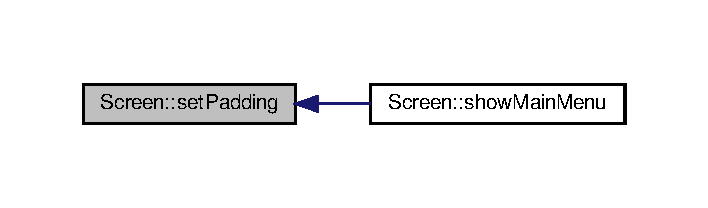
\includegraphics[width=340pt]{classScreen_a32771ff2a19f570bf35654e11971e938_icgraph}
\end{center}
\end{figure}
\mbox{\Hypertarget{classScreen_a16bd8465322e12b669e26ecccd4a3704}\label{classScreen_a16bd8465322e12b669e26ecccd4a3704}} 
\index{Screen@{Screen}!show\+Bar@{show\+Bar}}
\index{show\+Bar@{show\+Bar}!Screen@{Screen}}
\subsubsection{\texorpdfstring{show\+Bar()}{showBar()}}
{\footnotesize\ttfamily void Screen\+::show\+Bar (\begin{DoxyParamCaption}\item[{std\+::string}]{simbolo }\end{DoxyParamCaption})}

O método show\+Bar mostra a barra na tela.~\newline
Argumentos\+:
\begin{DoxyItemize}
\item title\+: texto do título;
\item simbolo\+: símbolo da barra.
\end{DoxyItemize}

Exceções\+:
\begin{DoxyItemize}
\item o comprimento da string simbolo não pode ser zero;
\end{DoxyItemize}Este é o diagrama das funções que utilizam esta função\+:\nopagebreak
\begin{figure}[H]
\begin{center}
\leavevmode
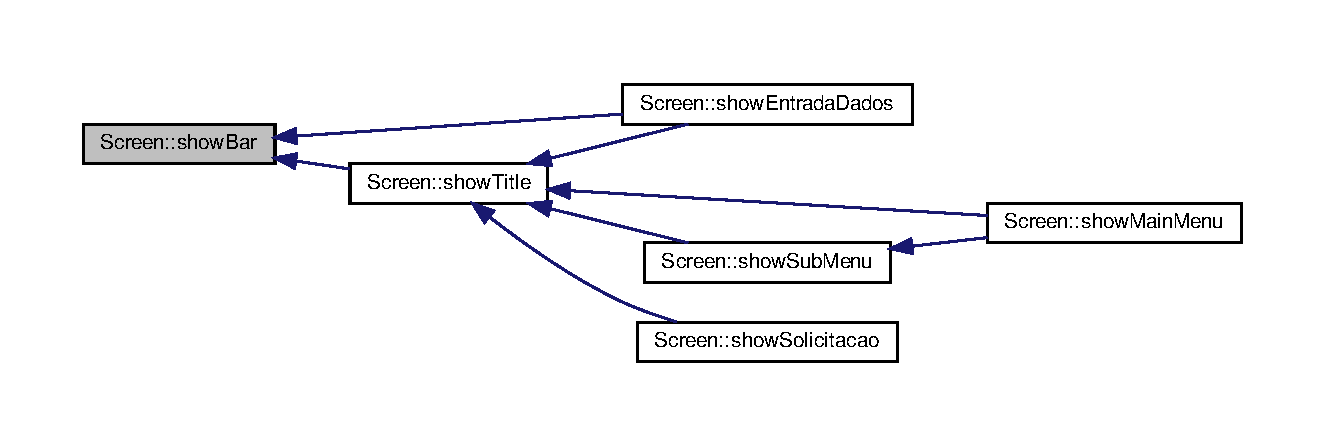
\includegraphics[width=350pt]{classScreen_a16bd8465322e12b669e26ecccd4a3704_icgraph}
\end{center}
\end{figure}
\mbox{\Hypertarget{classScreen_a7b425f6ea8830066c837f84e09f493a0}\label{classScreen_a7b425f6ea8830066c837f84e09f493a0}} 
\index{Screen@{Screen}!show\+Entrada\+Dados@{show\+Entrada\+Dados}}
\index{show\+Entrada\+Dados@{show\+Entrada\+Dados}!Screen@{Screen}}
\subsubsection{\texorpdfstring{show\+Entrada\+Dados()}{showEntradaDados()}}
{\footnotesize\ttfamily void Screen\+::show\+Entrada\+Dados (\begin{DoxyParamCaption}\item[{float \&}]{quantidade,  }\item[{int \&}]{cod\+\_\+origem,  }\item[{int \&}]{cod\+\_\+destino,  }\item[{int \&}]{num\+\_\+solicitacoes,  }\item[{int}]{num\+\_\+localidades }\end{DoxyParamCaption})}

O método show\+Entrada\+Dados mostra as solicitações de transporte e as opções de entrada de dados do sistema.~\newline
Argumentos\+:
\begin{DoxyItemize}
\item quantidade\+: quantidade de carga a ser transportada;
\item cod\+\_\+origem\+: código do município de origem;
\item cod\+\_\+destino\+: código do município de destino;
\item num\+\_\+solicitacoes\+: número corrente de solicitações; e
\item num\+\_\+localidades\+: número total de localidades carregadas para controle
\end{DoxyItemize}

Exceções\+:
\begin{DoxyItemize}
\item os valores de quantidade, número de solicitações e número de localidades deve ser maior que zero;
\item os valores dos códigos dos municípios de origem e destino não podem ser negativos;
\end{DoxyItemize}Grafo de chamadas desta função\+:\nopagebreak
\begin{figure}[H]
\begin{center}
\leavevmode
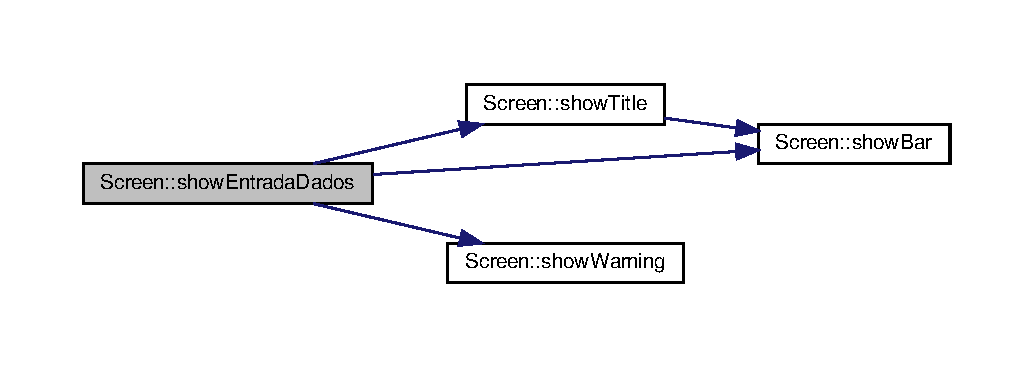
\includegraphics[width=350pt]{classScreen_a7b425f6ea8830066c837f84e09f493a0_cgraph}
\end{center}
\end{figure}
\mbox{\Hypertarget{classScreen_a3ea61b376ace3fa90b16ba31b01a8107}\label{classScreen_a3ea61b376ace3fa90b16ba31b01a8107}} 
\index{Screen@{Screen}!show\+Main\+Menu@{show\+Main\+Menu}}
\index{show\+Main\+Menu@{show\+Main\+Menu}!Screen@{Screen}}
\subsubsection{\texorpdfstring{show\+Main\+Menu()}{showMainMenu()}}
{\footnotesize\ttfamily void Screen\+::show\+Main\+Menu (\begin{DoxyParamCaption}\item[{\hyperlink{classScreen}{Screen} $\ast$}]{tela }\end{DoxyParamCaption})}

O método show\+Main\+Menu mostra o menu inicial do sistema.~\newline
Argumento\+:
\begin{DoxyItemize}
\item tela\+: objeto do tipo \hyperlink{classScreen}{Screen}
\end{DoxyItemize}

Exceções\+:
\begin{DoxyItemize}
\item argumento vazio
\end{DoxyItemize}Grafo de chamadas desta função\+:\nopagebreak
\begin{figure}[H]
\begin{center}
\leavevmode
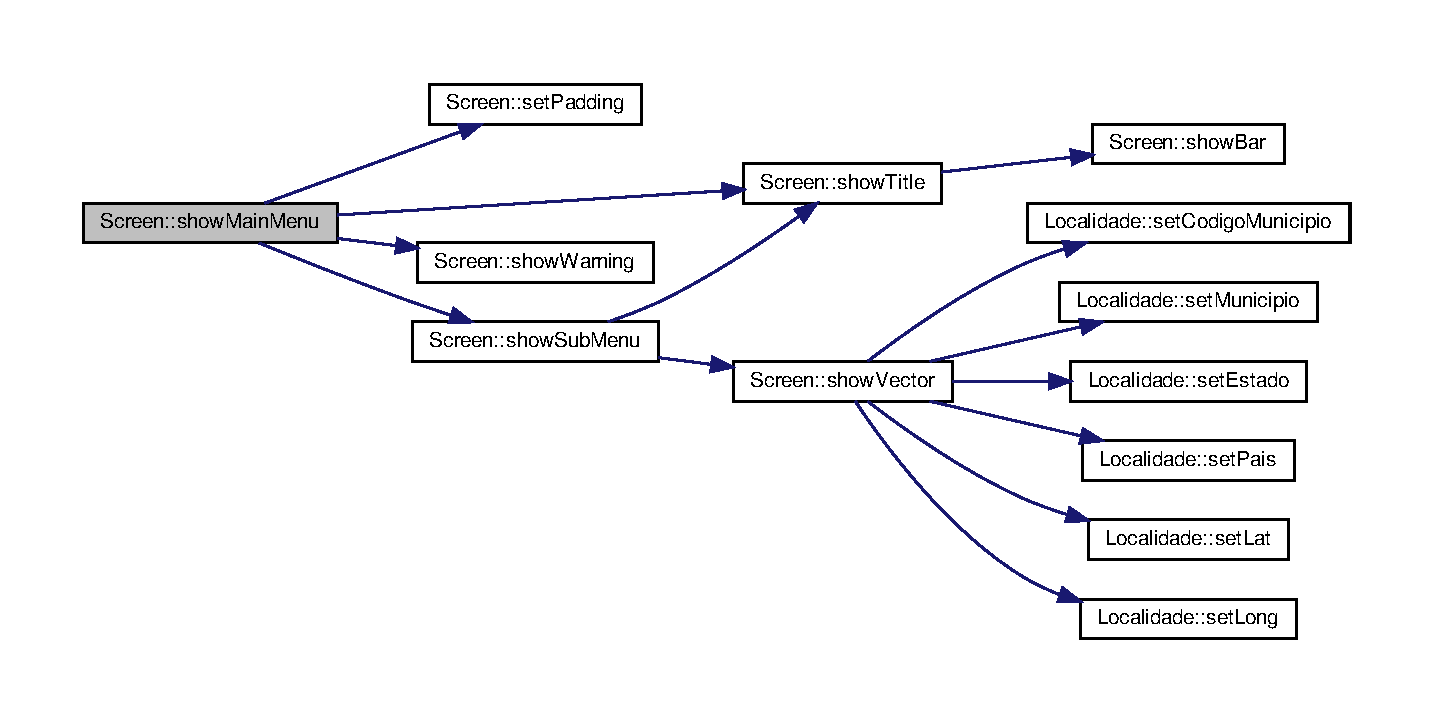
\includegraphics[width=350pt]{classScreen_a3ea61b376ace3fa90b16ba31b01a8107_cgraph}
\end{center}
\end{figure}
\mbox{\Hypertarget{classScreen_a2f514fb5d139b0b6e8d67c95ee6a2596}\label{classScreen_a2f514fb5d139b0b6e8d67c95ee6a2596}} 
\index{Screen@{Screen}!show\+Solicitacao@{show\+Solicitacao}}
\index{show\+Solicitacao@{show\+Solicitacao}!Screen@{Screen}}
\subsubsection{\texorpdfstring{show\+Solicitacao()}{showSolicitacao()}}
{\footnotesize\ttfamily void Screen\+::show\+Solicitacao (\begin{DoxyParamCaption}\item[{int}]{cod\+\_\+origem,  }\item[{int}]{cod\+\_\+destino,  }\item[{float}]{quantidade,  }\item[{std\+::vector$<$ \hyperlink{classLocalidade}{Localidade} $>$}]{vec\+\_\+local }\end{DoxyParamCaption})}

O método show\+Solicitacao mostra a solicitação na tela.~\newline
Argumentos\+:
\begin{DoxyItemize}
\item cod\+\_\+origem\+: código do município de origem;
\item cod\+\_\+destino\+: código do município de destino;
\item quantidade\+: quantidade de carga a ser transportada; e
\item vec\+\_\+local\+: número corrente de solicitações.
\end{DoxyItemize}

Exceções\+:
\begin{DoxyItemize}
\item o valor de quantidade deve ser maior que zero;
\item os valores dos códigos dos municípios de origem e destino não podem ser negativos;
\end{DoxyItemize}Grafo de chamadas desta função\+:\nopagebreak
\begin{figure}[H]
\begin{center}
\leavevmode
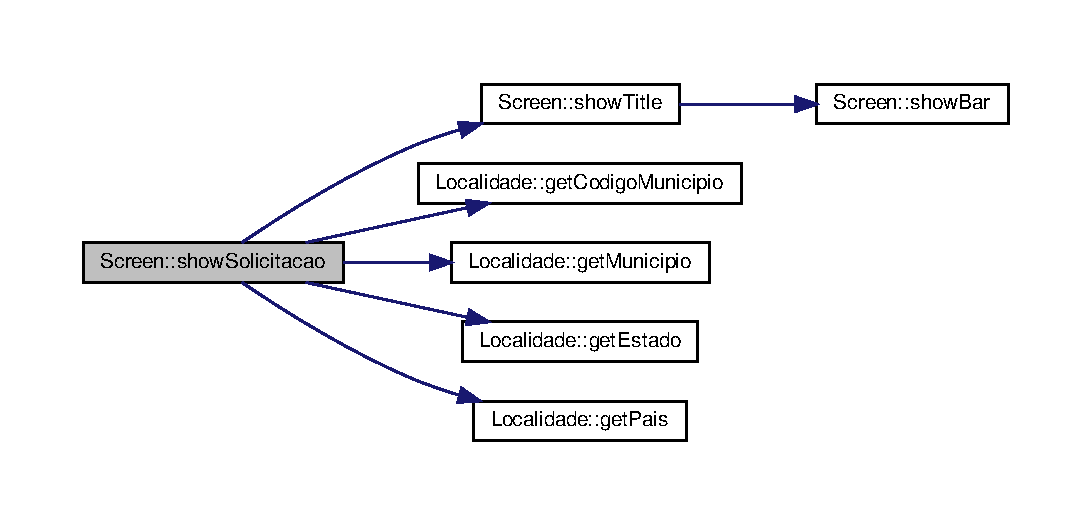
\includegraphics[width=350pt]{classScreen_a2f514fb5d139b0b6e8d67c95ee6a2596_cgraph}
\end{center}
\end{figure}
\mbox{\Hypertarget{classScreen_ac974e1d0dc9ab1f4c9be2d8f70d763c7}\label{classScreen_ac974e1d0dc9ab1f4c9be2d8f70d763c7}} 
\index{Screen@{Screen}!show\+Sub\+Menu@{show\+Sub\+Menu}}
\index{show\+Sub\+Menu@{show\+Sub\+Menu}!Screen@{Screen}}
\subsubsection{\texorpdfstring{show\+Sub\+Menu()}{showSubMenu()}}
{\footnotesize\ttfamily void Screen\+::show\+Sub\+Menu (\begin{DoxyParamCaption}{ }\end{DoxyParamCaption})}

O método show\+Sub\+Menu mostra o submenu com as opções de entrada de dados.~\newline
Sem argumento.Grafo de chamadas desta função\+:\nopagebreak
\begin{figure}[H]
\begin{center}
\leavevmode
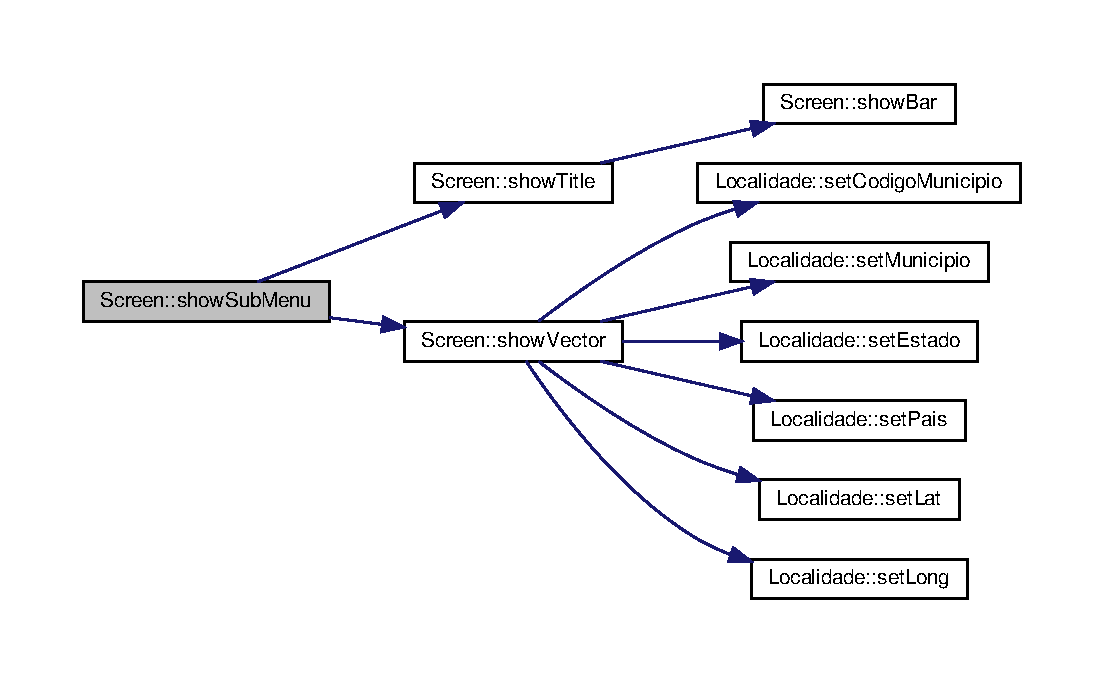
\includegraphics[width=350pt]{classScreen_ac974e1d0dc9ab1f4c9be2d8f70d763c7_cgraph}
\end{center}
\end{figure}
Este é o diagrama das funções que utilizam esta função\+:\nopagebreak
\begin{figure}[H]
\begin{center}
\leavevmode
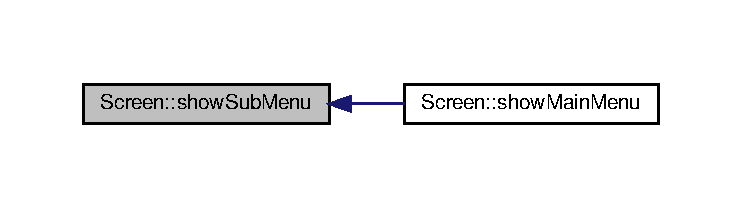
\includegraphics[width=350pt]{classScreen_ac974e1d0dc9ab1f4c9be2d8f70d763c7_icgraph}
\end{center}
\end{figure}
\mbox{\Hypertarget{classScreen_aefbd91aee5978143823031767159caf7}\label{classScreen_aefbd91aee5978143823031767159caf7}} 
\index{Screen@{Screen}!show\+Title@{show\+Title}}
\index{show\+Title@{show\+Title}!Screen@{Screen}}
\subsubsection{\texorpdfstring{show\+Title()}{showTitle()}}
{\footnotesize\ttfamily void Screen\+::show\+Title (\begin{DoxyParamCaption}\item[{std\+::string}]{titulo,  }\item[{std\+::string}]{simbolo }\end{DoxyParamCaption})}

O método show\+Title mostra o título formatado na tela.~\newline
Argumentos\+:
\begin{DoxyItemize}
\item title\+: texto do título;
\item simbolo\+: símbolo da barra.
\end{DoxyItemize}

Exceções\+:
\begin{DoxyItemize}
\item os comprimentos das strings não podem ser zero;
\end{DoxyItemize}Grafo de chamadas desta função\+:\nopagebreak
\begin{figure}[H]
\begin{center}
\leavevmode
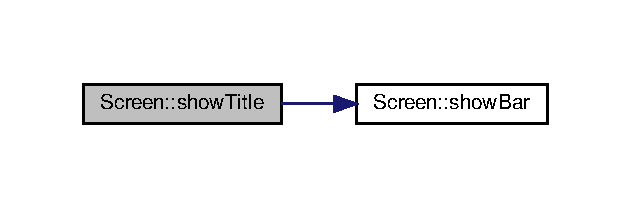
\includegraphics[width=303pt]{classScreen_aefbd91aee5978143823031767159caf7_cgraph}
\end{center}
\end{figure}
Este é o diagrama das funções que utilizam esta função\+:\nopagebreak
\begin{figure}[H]
\begin{center}
\leavevmode
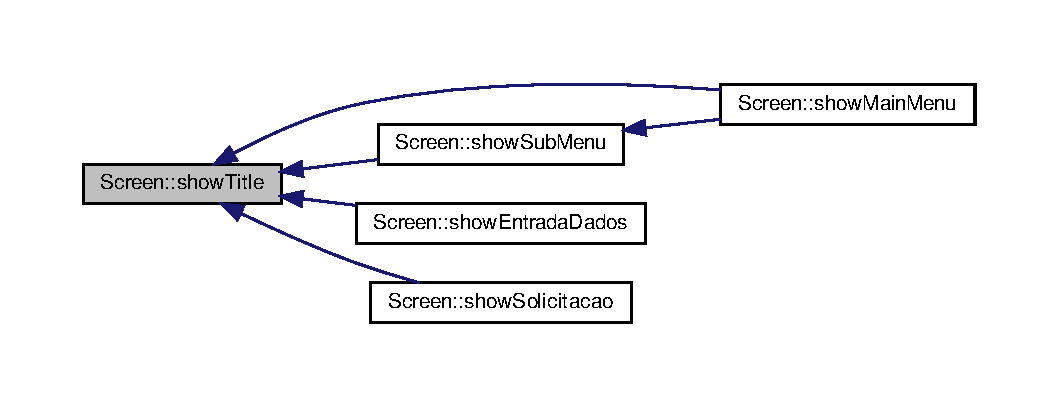
\includegraphics[width=350pt]{classScreen_aefbd91aee5978143823031767159caf7_icgraph}
\end{center}
\end{figure}
\mbox{\Hypertarget{classScreen_aca2a46f65496651c74b66e807f7ed421}\label{classScreen_aca2a46f65496651c74b66e807f7ed421}} 
\index{Screen@{Screen}!show\+Vector@{show\+Vector}}
\index{show\+Vector@{show\+Vector}!Screen@{Screen}}
\subsubsection{\texorpdfstring{show\+Vector()}{showVector()}}
{\footnotesize\ttfamily void Screen\+::show\+Vector (\begin{DoxyParamCaption}\item[{int}]{columns }\end{DoxyParamCaption})}

O método show\+Vector mostra as localidades carregadas do arquivo de localidades.~\newline
Argumentos\+:
\begin{DoxyItemize}
\item columns\+: número de colunas.
\end{DoxyItemize}

Exceções\+:
\begin{DoxyItemize}
\item o valor da variável columns de ser maior que zero;
\end{DoxyItemize}Grafo de chamadas desta função\+:\nopagebreak
\begin{figure}[H]
\begin{center}
\leavevmode
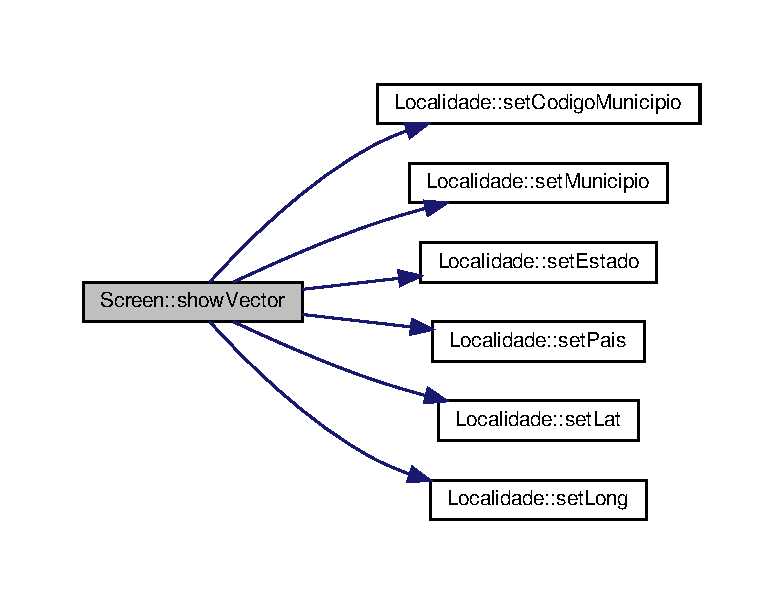
\includegraphics[width=350pt]{classScreen_aca2a46f65496651c74b66e807f7ed421_cgraph}
\end{center}
\end{figure}
Este é o diagrama das funções que utilizam esta função\+:\nopagebreak
\begin{figure}[H]
\begin{center}
\leavevmode
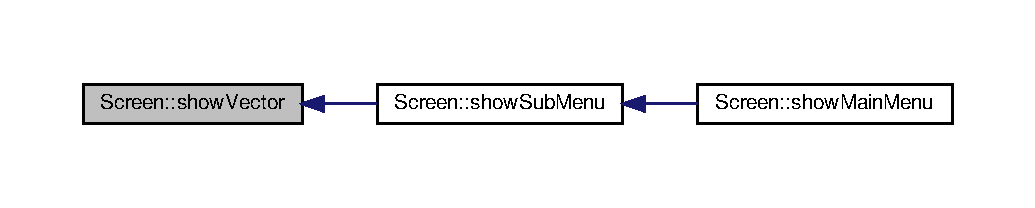
\includegraphics[width=350pt]{classScreen_aca2a46f65496651c74b66e807f7ed421_icgraph}
\end{center}
\end{figure}
\mbox{\Hypertarget{classScreen_a5fc8c4449368a8507f03bf3243677f1e}\label{classScreen_a5fc8c4449368a8507f03bf3243677f1e}} 
\index{Screen@{Screen}!show\+Warning@{show\+Warning}}
\index{show\+Warning@{show\+Warning}!Screen@{Screen}}
\subsubsection{\texorpdfstring{show\+Warning()}{showWarning()}}
{\footnotesize\ttfamily void Screen\+::show\+Warning (\begin{DoxyParamCaption}\item[{std\+::string}]{aviso }\end{DoxyParamCaption})}

O método show\+Solicitacao mostra a solicitação na tela.~\newline
Argumentos\+:
\begin{DoxyItemize}
\item cod\+\_\+origem\+: código do município de origem;
\item cod\+\_\+destino\+: código do município de destino;
\item quantidade\+: quantidade de carga a ser transportada; e
\item vec\+\_\+local\+: número corrente de solicitações.
\end{DoxyItemize}

Exceções\+:
\begin{DoxyItemize}
\item o valor de quantidade deve ser maior que zero;
\item os valores dos códigos dos municípios de origem e destino não podem ser negativos;
\end{DoxyItemize}Este é o diagrama das funções que utilizam esta função\+:\nopagebreak
\begin{figure}[H]
\begin{center}
\leavevmode
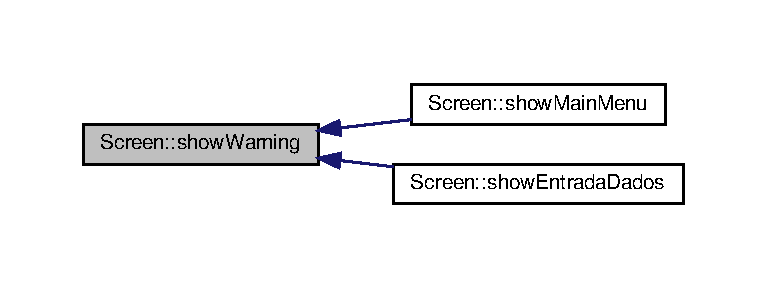
\includegraphics[width=350pt]{classScreen_a5fc8c4449368a8507f03bf3243677f1e_icgraph}
\end{center}
\end{figure}


A documentação para esta classe foi gerada a partir dos seguintes ficheiros\+:\begin{DoxyCompactItemize}
\item 
include/tools.\+hpp\item 
src/tools.\+cpp\end{DoxyCompactItemize}

\hypertarget{classSolicitacao}{}\section{Referência à classe Solicitacao}
\label{classSolicitacao}\index{Solicitacao@{Solicitacao}}


Esta classe representa uma solicitação de transporte de uma determinada quantidade de carga entre duas localidades.  




{\ttfamily \#include $<$solicitacao.\+hpp$>$}

\subsection*{Membros públicos}
\begin{DoxyCompactItemize}
\item 
\hyperlink{classSolicitacao_a67c9ab7bb3295e4a5a0933486f7e0f4b}{Solicitacao} ()
\item 
\hyperlink{classSolicitacao_a7488a91778013e8666db5f3dde061e2c}{Solicitacao} (int, int, float)
\item 
void \hyperlink{classSolicitacao_a585f55cfa44c1e16d535935eead17f44}{set\+Origem} (int)
\item 
void \hyperlink{classSolicitacao_ac772a2517a1d395f1a541424d29716cd}{set\+Destino} (int)
\item 
void \hyperlink{classSolicitacao_acf1db9c6843df635aca0bbacae8cf7c7}{set\+Quantidade} (float quantidade)
\item 
int \hyperlink{classSolicitacao_a53a5b37dd6aca895d84ef9991fc7775b}{get\+Origem} ()
\item 
int \hyperlink{classSolicitacao_a8448e5d5b0ca18b7e8ff022415ec6836}{get\+Destino} ()
\item 
float \hyperlink{classSolicitacao_a7e936983b3b1c6d4010649edcbac4819}{get\+Quantidade} ()
\end{DoxyCompactItemize}


\subsection{Descrição detalhada}
Esta classe representa uma solicitação de transporte de uma determinada quantidade de carga entre duas localidades. 

\subsection{Documentação dos Construtores \& Destrutor}
\mbox{\Hypertarget{classSolicitacao_a67c9ab7bb3295e4a5a0933486f7e0f4b}\label{classSolicitacao_a67c9ab7bb3295e4a5a0933486f7e0f4b}} 
\index{Solicitacao@{Solicitacao}!Solicitacao@{Solicitacao}}
\index{Solicitacao@{Solicitacao}!Solicitacao@{Solicitacao}}
\subsubsection{\texorpdfstring{Solicitacao()}{Solicitacao()}\hspace{0.1cm}{\footnotesize\ttfamily [1/2]}}
{\footnotesize\ttfamily Solicitacao\+::\+Solicitacao (\begin{DoxyParamCaption}{ }\end{DoxyParamCaption})}

Construtor sem argumentos da classe \hyperlink{classRodoviario}{Rodoviario}\mbox{\Hypertarget{classSolicitacao_a7488a91778013e8666db5f3dde061e2c}\label{classSolicitacao_a7488a91778013e8666db5f3dde061e2c}} 
\index{Solicitacao@{Solicitacao}!Solicitacao@{Solicitacao}}
\index{Solicitacao@{Solicitacao}!Solicitacao@{Solicitacao}}
\subsubsection{\texorpdfstring{Solicitacao()}{Solicitacao()}\hspace{0.1cm}{\footnotesize\ttfamily [2/2]}}
{\footnotesize\ttfamily Solicitacao\+::\+Solicitacao (\begin{DoxyParamCaption}\item[{int}]{origem,  }\item[{int}]{destino,  }\item[{float}]{quantidade }\end{DoxyParamCaption})}

Construtor da classe \hyperlink{classModal}{Modal}~\newline
Argumentos\+:
\begin{DoxyItemize}
\item origem\+: código do município de origem;
\item destino\+: código do município de destino;
\item quantidade\+: valor da quantidade de carga, em toneladas.
\end{DoxyItemize}

Exceção\+:
\begin{DoxyItemize}
\item os valores não podem ser negativos e o valor da carga não pode ser zero;
\end{DoxyItemize}

\subsection{Documentação dos métodos}
\mbox{\Hypertarget{classSolicitacao_a8448e5d5b0ca18b7e8ff022415ec6836}\label{classSolicitacao_a8448e5d5b0ca18b7e8ff022415ec6836}} 
\index{Solicitacao@{Solicitacao}!get\+Destino@{get\+Destino}}
\index{get\+Destino@{get\+Destino}!Solicitacao@{Solicitacao}}
\subsubsection{\texorpdfstring{get\+Destino()}{getDestino()}}
{\footnotesize\ttfamily int Solicitacao\+::get\+Destino (\begin{DoxyParamCaption}{ }\end{DoxyParamCaption})}

Retorna o código do município de destino.~\newline
Sem argumentos.\mbox{\Hypertarget{classSolicitacao_a53a5b37dd6aca895d84ef9991fc7775b}\label{classSolicitacao_a53a5b37dd6aca895d84ef9991fc7775b}} 
\index{Solicitacao@{Solicitacao}!get\+Origem@{get\+Origem}}
\index{get\+Origem@{get\+Origem}!Solicitacao@{Solicitacao}}
\subsubsection{\texorpdfstring{get\+Origem()}{getOrigem()}}
{\footnotesize\ttfamily int Solicitacao\+::get\+Origem (\begin{DoxyParamCaption}{ }\end{DoxyParamCaption})}

Retorna o código do município de origem.~\newline
Sem argumentos.\mbox{\Hypertarget{classSolicitacao_a7e936983b3b1c6d4010649edcbac4819}\label{classSolicitacao_a7e936983b3b1c6d4010649edcbac4819}} 
\index{Solicitacao@{Solicitacao}!get\+Quantidade@{get\+Quantidade}}
\index{get\+Quantidade@{get\+Quantidade}!Solicitacao@{Solicitacao}}
\subsubsection{\texorpdfstring{get\+Quantidade()}{getQuantidade()}}
{\footnotesize\ttfamily float Solicitacao\+::get\+Quantidade (\begin{DoxyParamCaption}{ }\end{DoxyParamCaption})}

Retorna o valor da quantidade de carga a ser transportada.~\newline
Sem argumentos.\mbox{\Hypertarget{classSolicitacao_ac772a2517a1d395f1a541424d29716cd}\label{classSolicitacao_ac772a2517a1d395f1a541424d29716cd}} 
\index{Solicitacao@{Solicitacao}!set\+Destino@{set\+Destino}}
\index{set\+Destino@{set\+Destino}!Solicitacao@{Solicitacao}}
\subsubsection{\texorpdfstring{set\+Destino()}{setDestino()}}
{\footnotesize\ttfamily void Solicitacao\+::set\+Destino (\begin{DoxyParamCaption}\item[{int}]{destino }\end{DoxyParamCaption})}

Atribui o valor do código do município de destino.~\newline
 Argumento\+:
\begin{DoxyItemize}
\item destino\+: código do município de destino
\end{DoxyItemize}

Exceção\+:
\begin{DoxyItemize}
\item o valor não pode ser negativo;
\end{DoxyItemize}\mbox{\Hypertarget{classSolicitacao_a585f55cfa44c1e16d535935eead17f44}\label{classSolicitacao_a585f55cfa44c1e16d535935eead17f44}} 
\index{Solicitacao@{Solicitacao}!set\+Origem@{set\+Origem}}
\index{set\+Origem@{set\+Origem}!Solicitacao@{Solicitacao}}
\subsubsection{\texorpdfstring{set\+Origem()}{setOrigem()}}
{\footnotesize\ttfamily void Solicitacao\+::set\+Origem (\begin{DoxyParamCaption}\item[{int}]{origem }\end{DoxyParamCaption})}

Atribui o valor do código do município de origem.~\newline
 Argumento\+:
\begin{DoxyItemize}
\item origem\+: código do município de origem
\end{DoxyItemize}

Exceção\+:
\begin{DoxyItemize}
\item o valor não pode ser negativo;
\end{DoxyItemize}\mbox{\Hypertarget{classSolicitacao_acf1db9c6843df635aca0bbacae8cf7c7}\label{classSolicitacao_acf1db9c6843df635aca0bbacae8cf7c7}} 
\index{Solicitacao@{Solicitacao}!set\+Quantidade@{set\+Quantidade}}
\index{set\+Quantidade@{set\+Quantidade}!Solicitacao@{Solicitacao}}
\subsubsection{\texorpdfstring{set\+Quantidade()}{setQuantidade()}}
{\footnotesize\ttfamily void Solicitacao\+::set\+Quantidade (\begin{DoxyParamCaption}\item[{float}]{quantidade }\end{DoxyParamCaption})}

Atribui o valor da quantidade de carga a ser transportada.~\newline
 Argumento\+:
\begin{DoxyItemize}
\item quantidade\+: valor da quantidade de carga
\end{DoxyItemize}

Exceção\+:
\begin{DoxyItemize}
\item o valor não pode ser negativo;
\end{DoxyItemize}

A documentação para esta classe foi gerada a partir dos seguintes ficheiros\+:\begin{DoxyCompactItemize}
\item 
include/solicitacao.\+hpp\item 
src/solicitacao.\+cpp\end{DoxyCompactItemize}

%--- End generated contents ---

% Index
\backmatter
\newpage
\phantomsection
\clearemptydoublepage
\addcontentsline{toc}{chapter}{Índice}
\printindex

\end{document}
